\documentclass[12pt]{beamer}

%\includeonlyframes{current}

\usetheme[sectionpage=none, subsectionpage=progressbar, progressbar=foot, numbering=fraction]{metropolis}

\makeatletter
\setlength{\metropolis@frametitle@padding}{1.6ex}% <- default 2.2 ex

\setbeamertemplate{footline}{%
  \begin{beamercolorbox}[wd=\textwidth, sep=1.5ex]{footline}% <- default 3ex
    \usebeamerfont{page number in head/foot}%
    \usebeamertemplate*{frame footer}
    \hfill%
    \usebeamertemplate*{frame numbering}
  \end{beamercolorbox}%
}
\makeatother

\AtBeginSubsection
{
  \begin{frame}{Where are we?}
    \tableofcontents[sectionstyle=show/shaded, subsectionstyle=show/shaded/hide]
  \end{frame}
}

\makeatletter
\setbeamertemplate{headline}{
  \begin{beamercolorbox}{upper separation line head}
  \end{beamercolorbox}
  \begin{beamercolorbox}{section in head/foot}
    \vskip2pt\insertsectionnavigationhorizontal{\paperwidth}{}{}\vskip2pt
  \end{beamercolorbox}
  \begin{beamercolorbox}{lower separation line head}
  \end{beamercolorbox}
}
\makeatother
\setbeamercolor{section in head/foot}{fg=normal text.bg, bg=structure.fg}

\setbeamertemplate{itemize items}[square]


\usepackage{tabularx}
\usepackage{menukeys}
\usepackage{minted}


\title{Hacker Tools: \\Course Overview, Linux Install Fest, Virtual Machines}
\author{Julius Putra Tanu Setiaji}
\date{3 September 2019}

\begin{document}

\frame[plain]{\titlepage}

\section{Introduction}
\subsection{}

\begin{frame}{NUS Hackers}

  \begin{center}
    
\includegraphics[width=0.5\linewidth]{../NUSHackers}

    \url{http://nushackers.org}
  \end{center}

  \begin{center}
    \textbf{hacker}school

    Friday \textbf{Hacks}

    \textbf{Hack} \& Roll

    \textbf{Hacker} Tools
  \end{center}

\end{frame}

\begin{frame}{About Me}
  Hi! I'm Julius. My GitHub is \url{https://github.com/indocomsoft}

  A Year 3 Computer Science Undergraduate who loves hacking and building systems.

  I also enjoy Space Exploration, Music Theory and History.

    {\tiny (my favourite games are KSP and EU4 hit me up if you play those too)}
\end{frame}

\begin{frame}{Required Software}
  \begin{itemize}
    \item Download and install VirtualBox
    \item Download Ubuntu 19.04 ISO file
  \end{itemize}

  You can find the link to download both of these in our Facebook event page or our Telegram channel.
\end{frame}

\begin{frame}{What is a Hacker?}
  A \textbf{hacker} is someone who strives to solve problems in elegant and ingenious ways.

  Hack as in hackathon.

  Read more at \url{https://www.nushackers.org/why/}

  Examples: Richard Stallman, Linus Torvalds, Jamie Zawinski, Steve Wozniak, Ken Thompson, Dennis Ritchie
\end{frame}

\begin{frame}{Hacker Tools}
  Inspired by \url{https://hacker-tools.github.io/}, organised by SIPB at MIT.

  Learn to make the most of the tools that hackers have been using for decades.

  In this class, we'll help you learn how to make the most of tools that productive programmers use.
\end{frame}

\begin{frame}{Course Overview}
  \begin{center}
    \begin{tabularx}{\textwidth}{l|l|X}
      \textbf{Week} & \textbf{Date \& Time, Venue} & \textbf{Topic}                      \\ \hline
      4             & 3/9/19 6.30pm, SR1           & Linux Install Fest, Virtual Machine \\ \hline
      5             & 10/9/19 6.30pm, SR10         & Shell \& Scripting                  \\ \hline
      6             & 17/9/19 7pm, SR1             & Command Line Environment            \\ \hline
      8             & 8/10/19 6.30pm, SR1          & Data Wrangling                      \\ \hline
      9             & 15/10/19 6.30pm, SR1         & Web Browsers \& Privacy             \\ \hline
      10            & 22/10/19 6pm, SR1            & Editors (vim \& emacs)              \\ \hline
      11            & 29/10/19 6.30pm, SR1         & OS Customisation                    \\ \hline
      12            & 5/11/19 6.30pm, SR1          & \LaTeX                              \\ \hline
    \end{tabularx}
  \end{center}
\end{frame}

\section{Linux \& Virtual Machines}
\subsection{Brief Introduction to Linux \& Unix}

\begin{frame}{What is Linux?}
  Can that be eaten? \pause

  A Unix-like operating system kernel\only<2->{\footnote{The most fundamental part of an operating system -- it is a bridge between other software running on the computer and the hardware}}.

  The most popular kernel in the world!

  Android, Chromebooks, most routers, most servers, supercomputers
\end{frame}

\begin{frame}{What is Unix?}
  A family of multi-tasking, multi-user operating system, first released in 1973.

  The first popular multi-user Windows was Windows 2000!

  Examples: macOS, iOS, SunOS/Solaris, BSD, AIX, HP-UX

  Most popular family of operating systems in the world!
\end{frame}

\begin{frame}{Most Popular OS Family in the world!}
  \begin{center}
    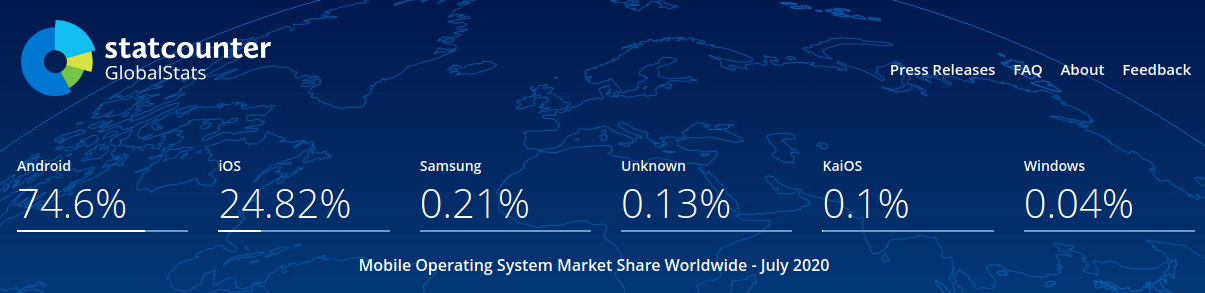
\includegraphics[width=0.75\linewidth]{phone-share}
  \end{center}

  \begin{columns}
    \begin{column}{0.5\linewidth}
      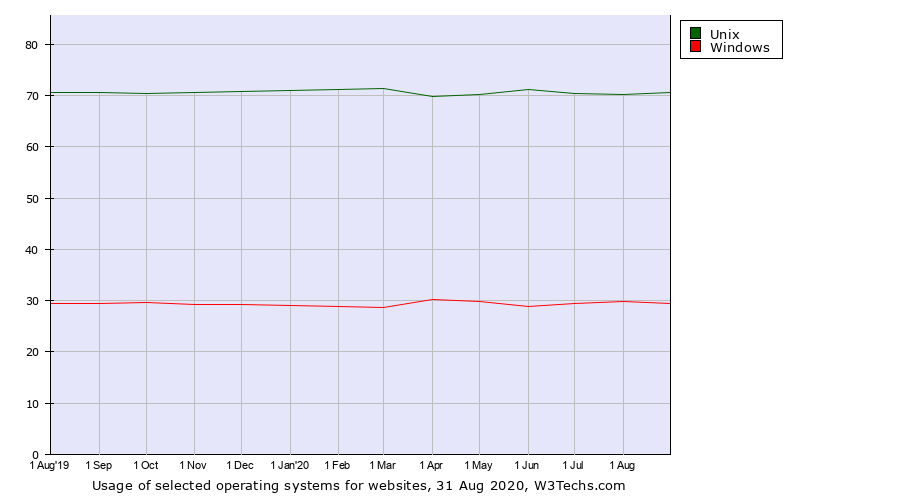
\includegraphics[width=\linewidth]{server}
    \end{column}
    \begin{column}{0.5\linewidth}
      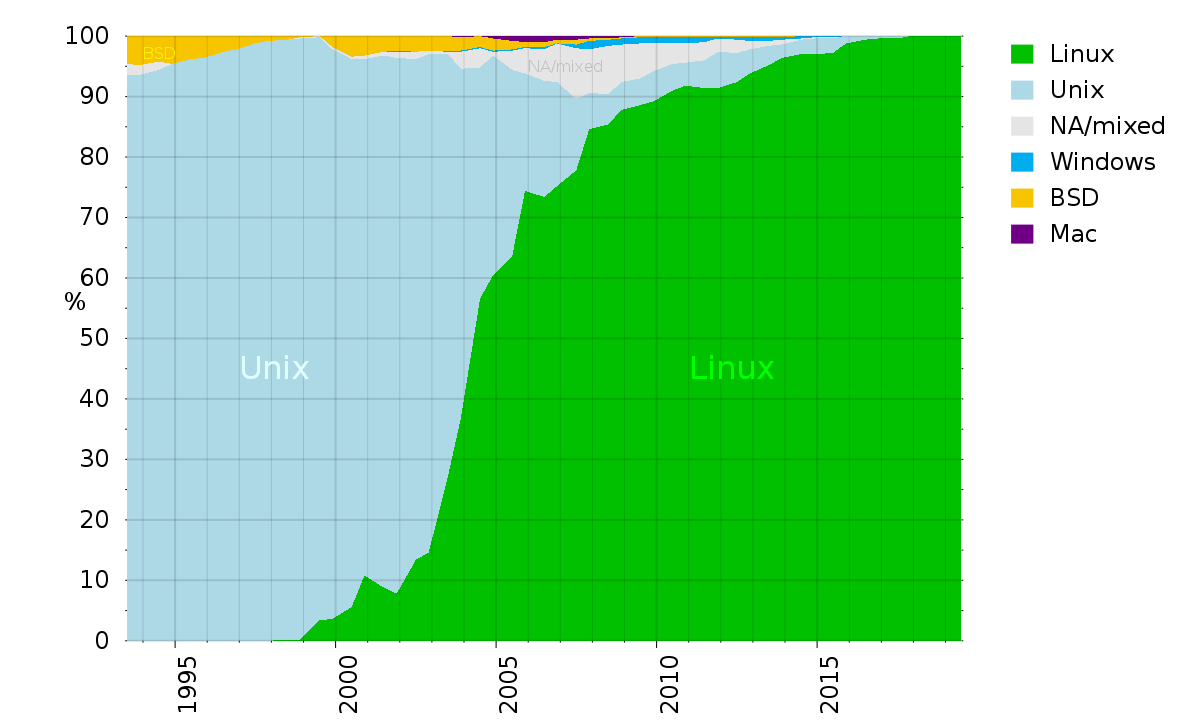
\includegraphics[width=\linewidth]{supercomputer}
    \end{column}
  \end{columns}
\end{frame}

\begin{frame}{Why should I use Linux?}
  Most development tools are designed around Unix, so the development experience is better!

  Useful skill: most technology companies use Unix.

  If you are a computing student, sooner or later you will end up developing for/on a Unix-like platform
\end{frame}

\subsection{Virtual Machine: What? Why?}
\begin{frame}{What is a VM?}
  Virtual machines are simulated computer.

  You can configure a guest virtual machine with some operating system and configuration and use it without affecting your host environment.
\end{frame}

\begin{frame}{Why use a VM?}
  Experiment with operating systems, software, and configurations without risk.

  For running software that only runs on a certain operating system.

  For experimenting with potentially malicious software.
\end{frame}

\begin{frame}{Useful Features}
  \textbf{Isolation}

  Isolating the guest from the host, so you can use VMs to run buggy or untrusted software reasonably safely.

  \textbf{Snapshots}

  Snapshots capture the entire machine state.

  You can make changes to your machine, and then restore to an earlier state.

\end{frame}

\begin{frame}{Disadvantages}
  VMs are generally slower than running on bare metal.

  Competes for resource with the host OS.

  May be unsuitable for certain applications, e.g. Games, High Performance Computing.
\end{frame}

\begin{frame}{Examples}
  \begin{columns}
    \begin{column}{0.33\linewidth}
      \begin{center}
        
\includegraphics[width=0.8\linewidth]{parallels}
      \end{center}
    \end{column}
    \begin{column}{0.33\linewidth}
      
\includegraphics[width=\linewidth]{hyperv}
    \end{column}
    \begin{column}{0.33\linewidth}
      
\includegraphics[width=\linewidth]{vmware}
    \end{column}
  \end{columns}
  \begin{columns}
    \begin{column}{0.5\linewidth}
      
\includegraphics[width=\linewidth]{qemu}
    \end{column}
    \begin{column}{0.5\linewidth}
      \begin{center}
        
\includegraphics[width=0.7\linewidth]{virtualbox}
      \end{center}
    \end{column}
  \end{columns}
\end{frame}

\subsection{Virtual Machine: Setting up}
\begin{frame}{Why VirtualBox?}
  \begin{center}
    
\includegraphics[width=0.25\linewidth]{virtualbox}
  \end{center}

  We are going to use VirtualBox, because:
  \begin{itemize}
    \item It is FOSS (Free Open Source Software)
    \item It has a GUI (Graphical User Interface)
    \item It is cross-platform
  \end{itemize}

  Possible disadvantages: owned by Oracle, quite power-hungry (on macOS)
\end{frame}

\begin{frame}{VirtualBox main UI}
  \begin{center}
    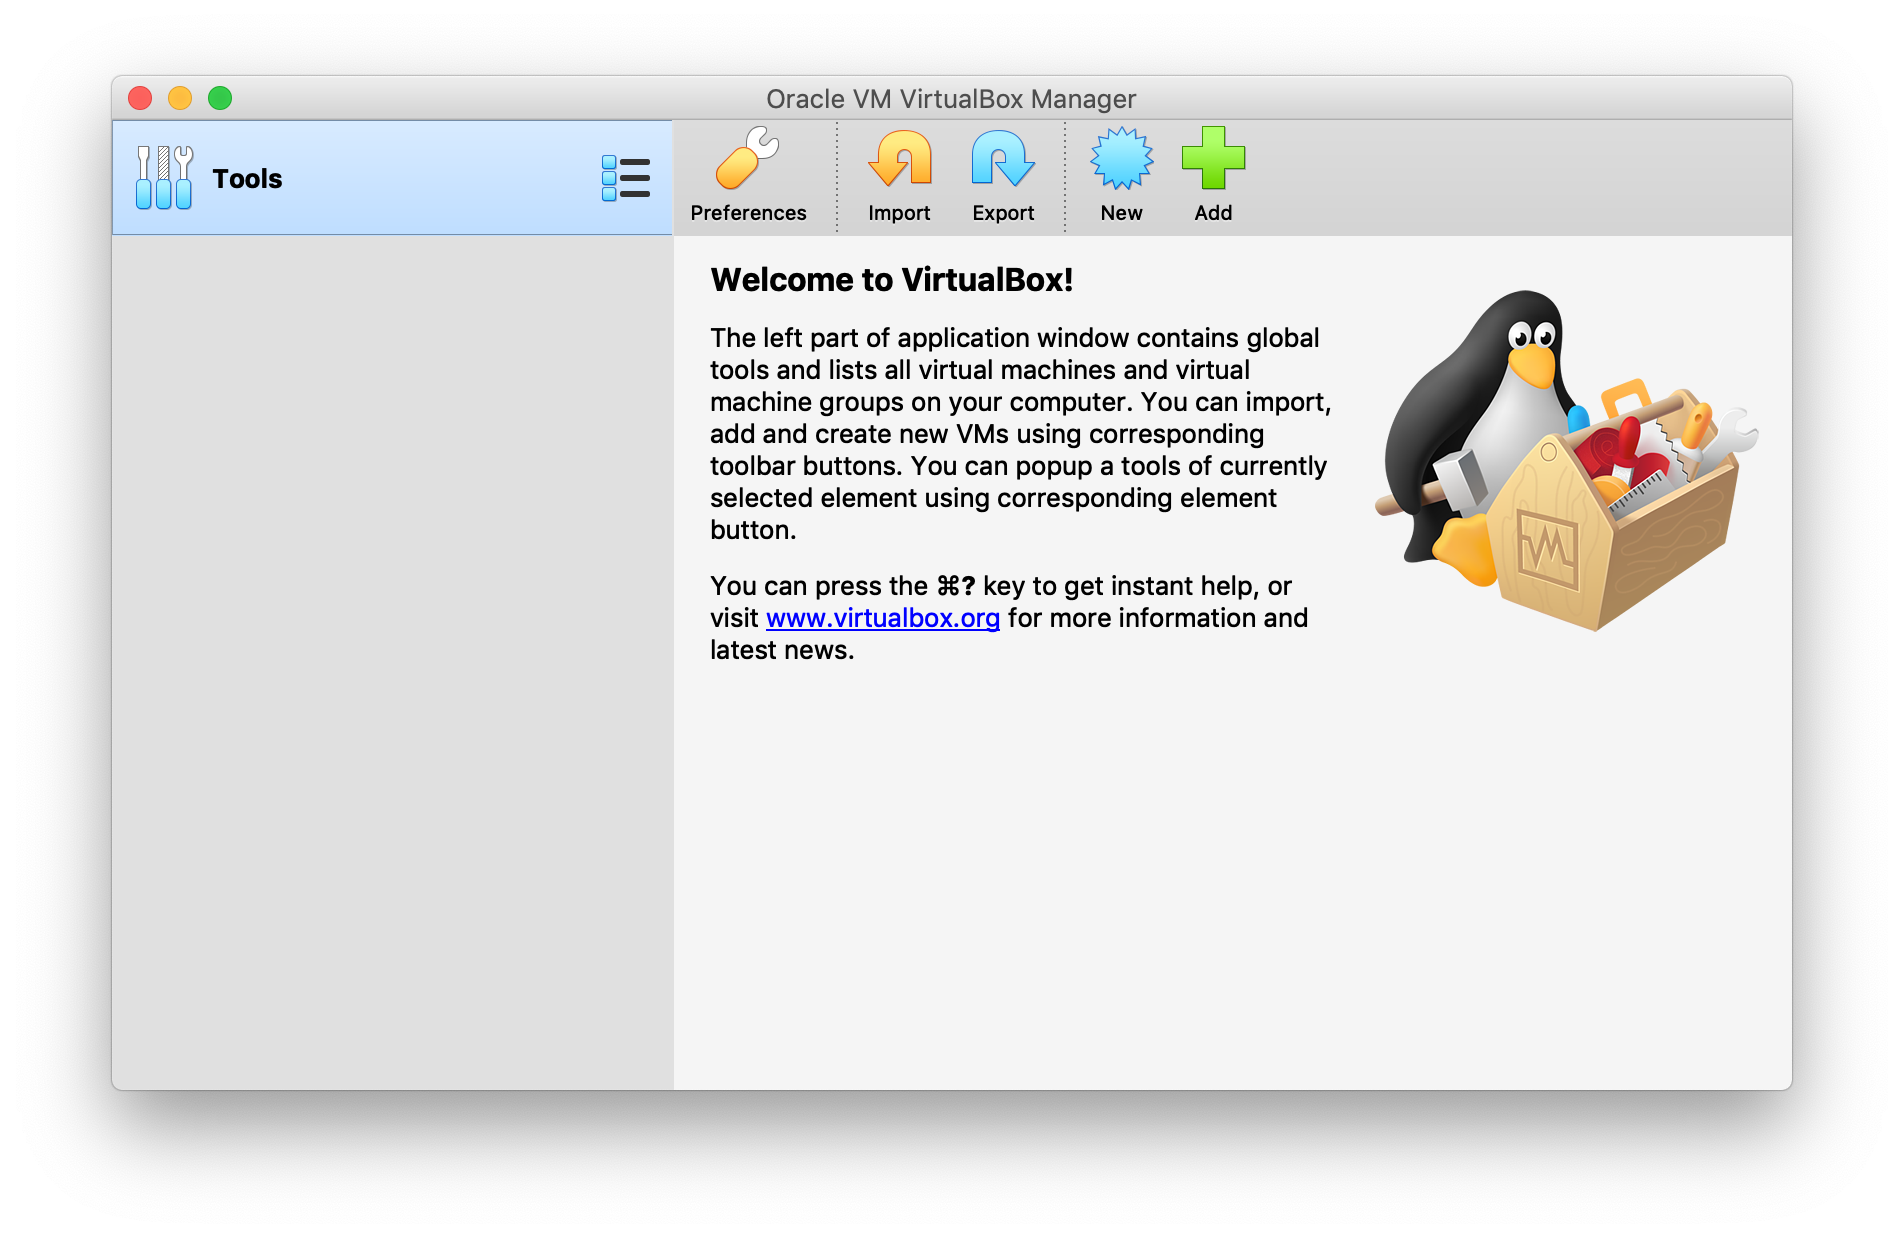
\includegraphics[width=0.8\linewidth]{vb-main}
  \end{center}
  Click on ``Add''
\end{frame}

\begin{frame}{Creating new VM}
  \begin{center}
    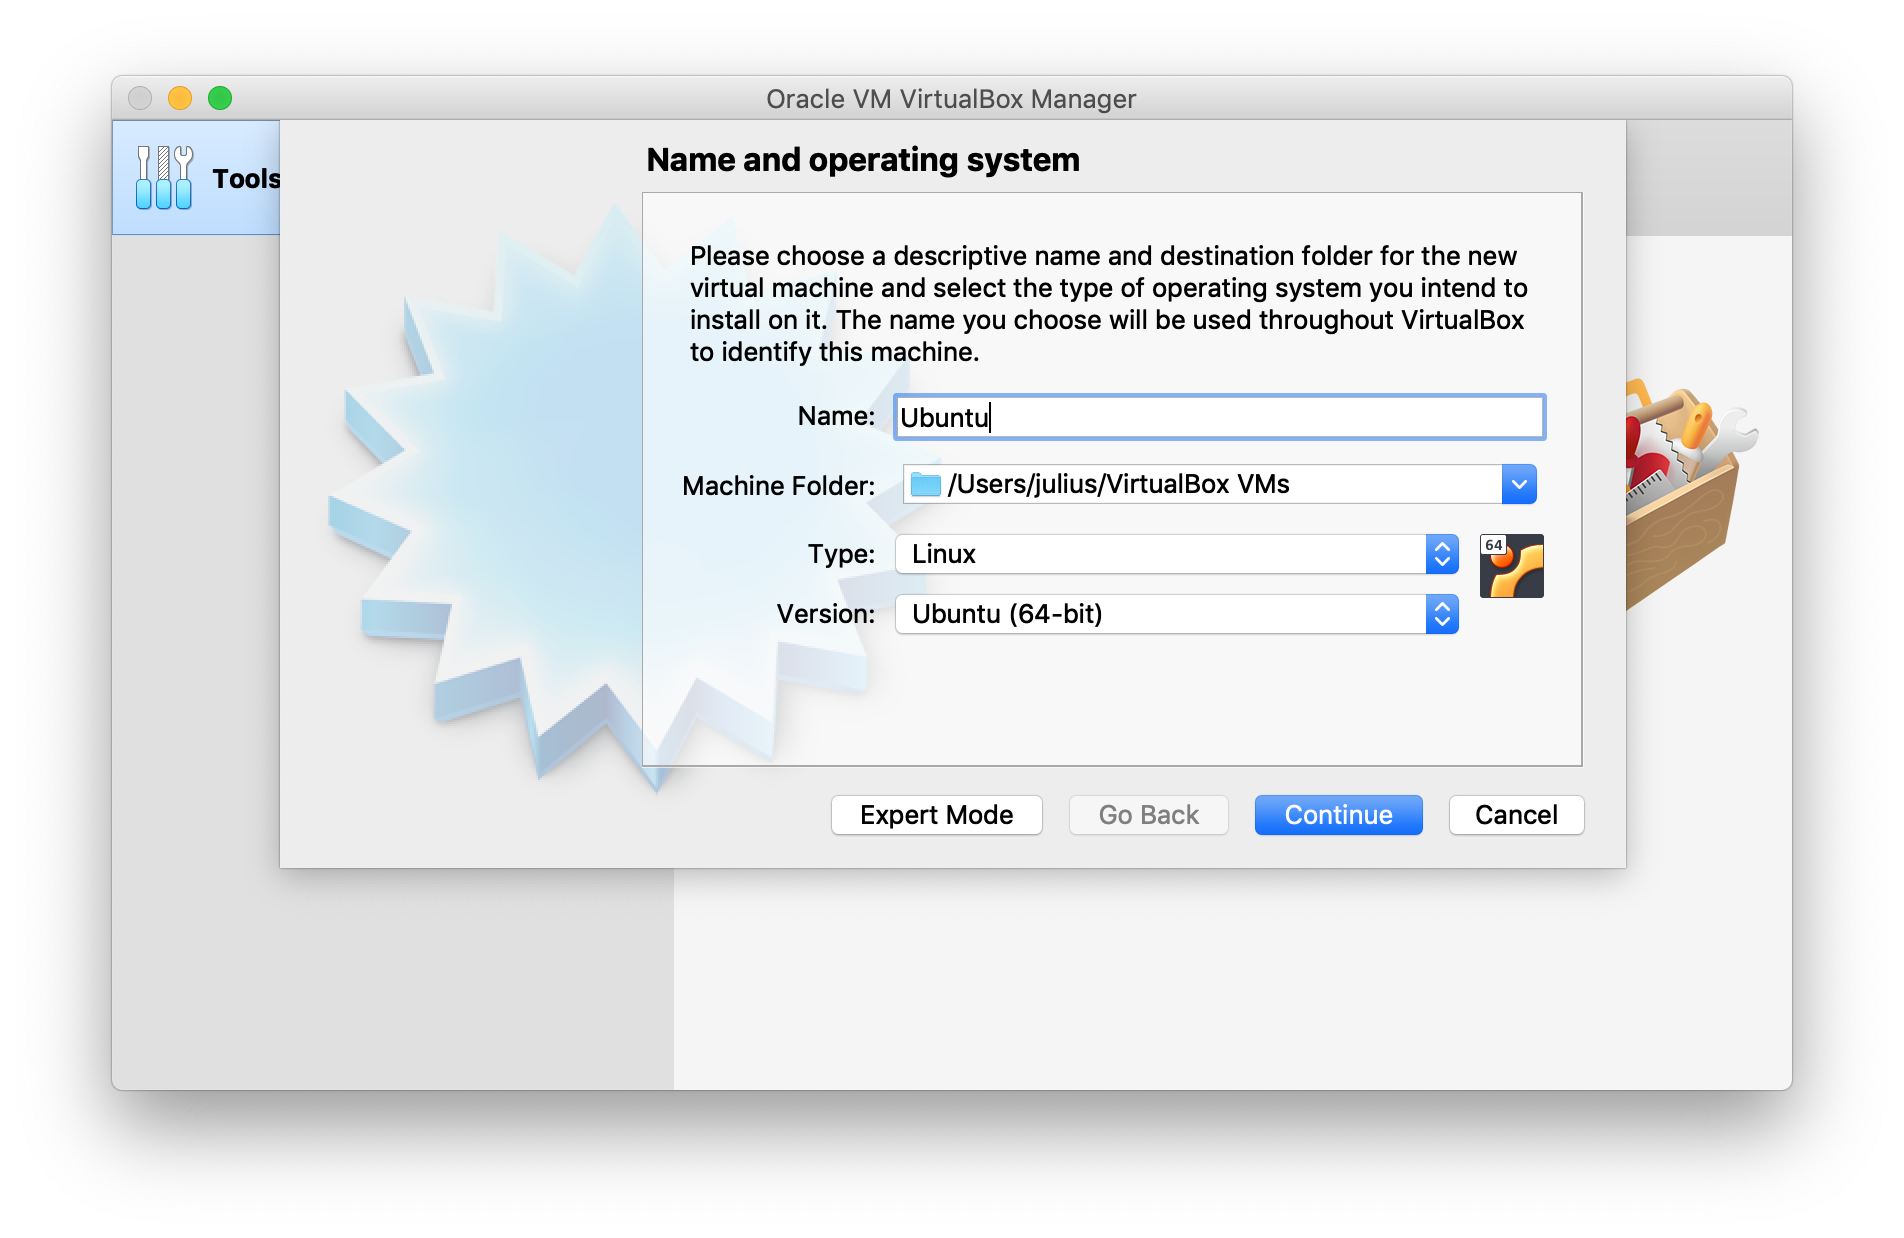
\includegraphics[width=0.8\linewidth]{vb-new}
  \end{center}
  Use Ubuntu as the name, VirtualBox should detect the type and variation automagically.
\end{frame}

\begin{frame}{Set amount of memory allocated}
  \begin{center}
    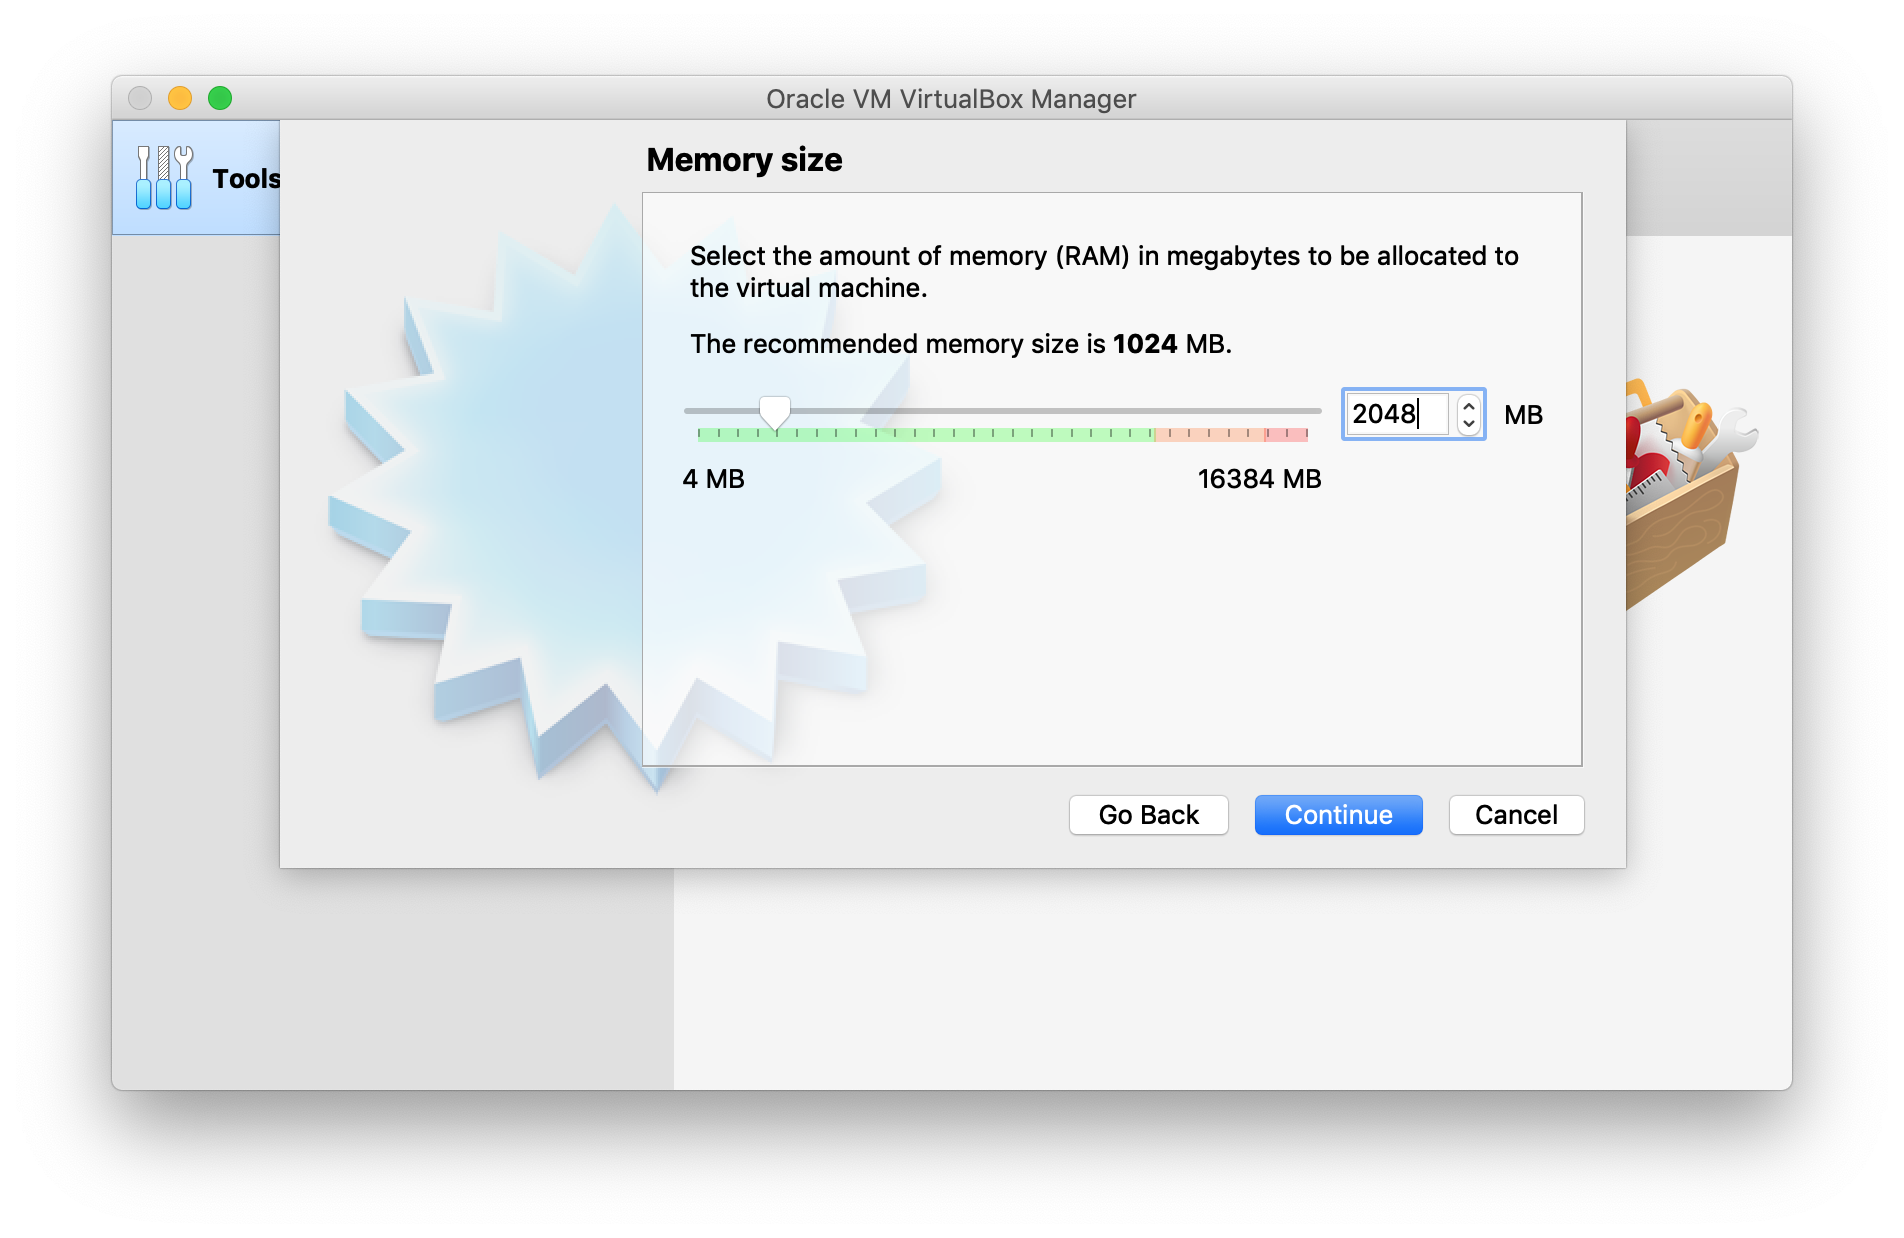
\includegraphics[width=0.8\linewidth]{vb-mem}
  \end{center}
  Ubuntu has a minimum of 512 MiB and recommends 2 GiB, but in general do not exceed 1/4 of the amount of physical RAM available.
\end{frame}

\begin{frame}{Create Virtual Hard Disk (1/4)}
  \begin{center}
    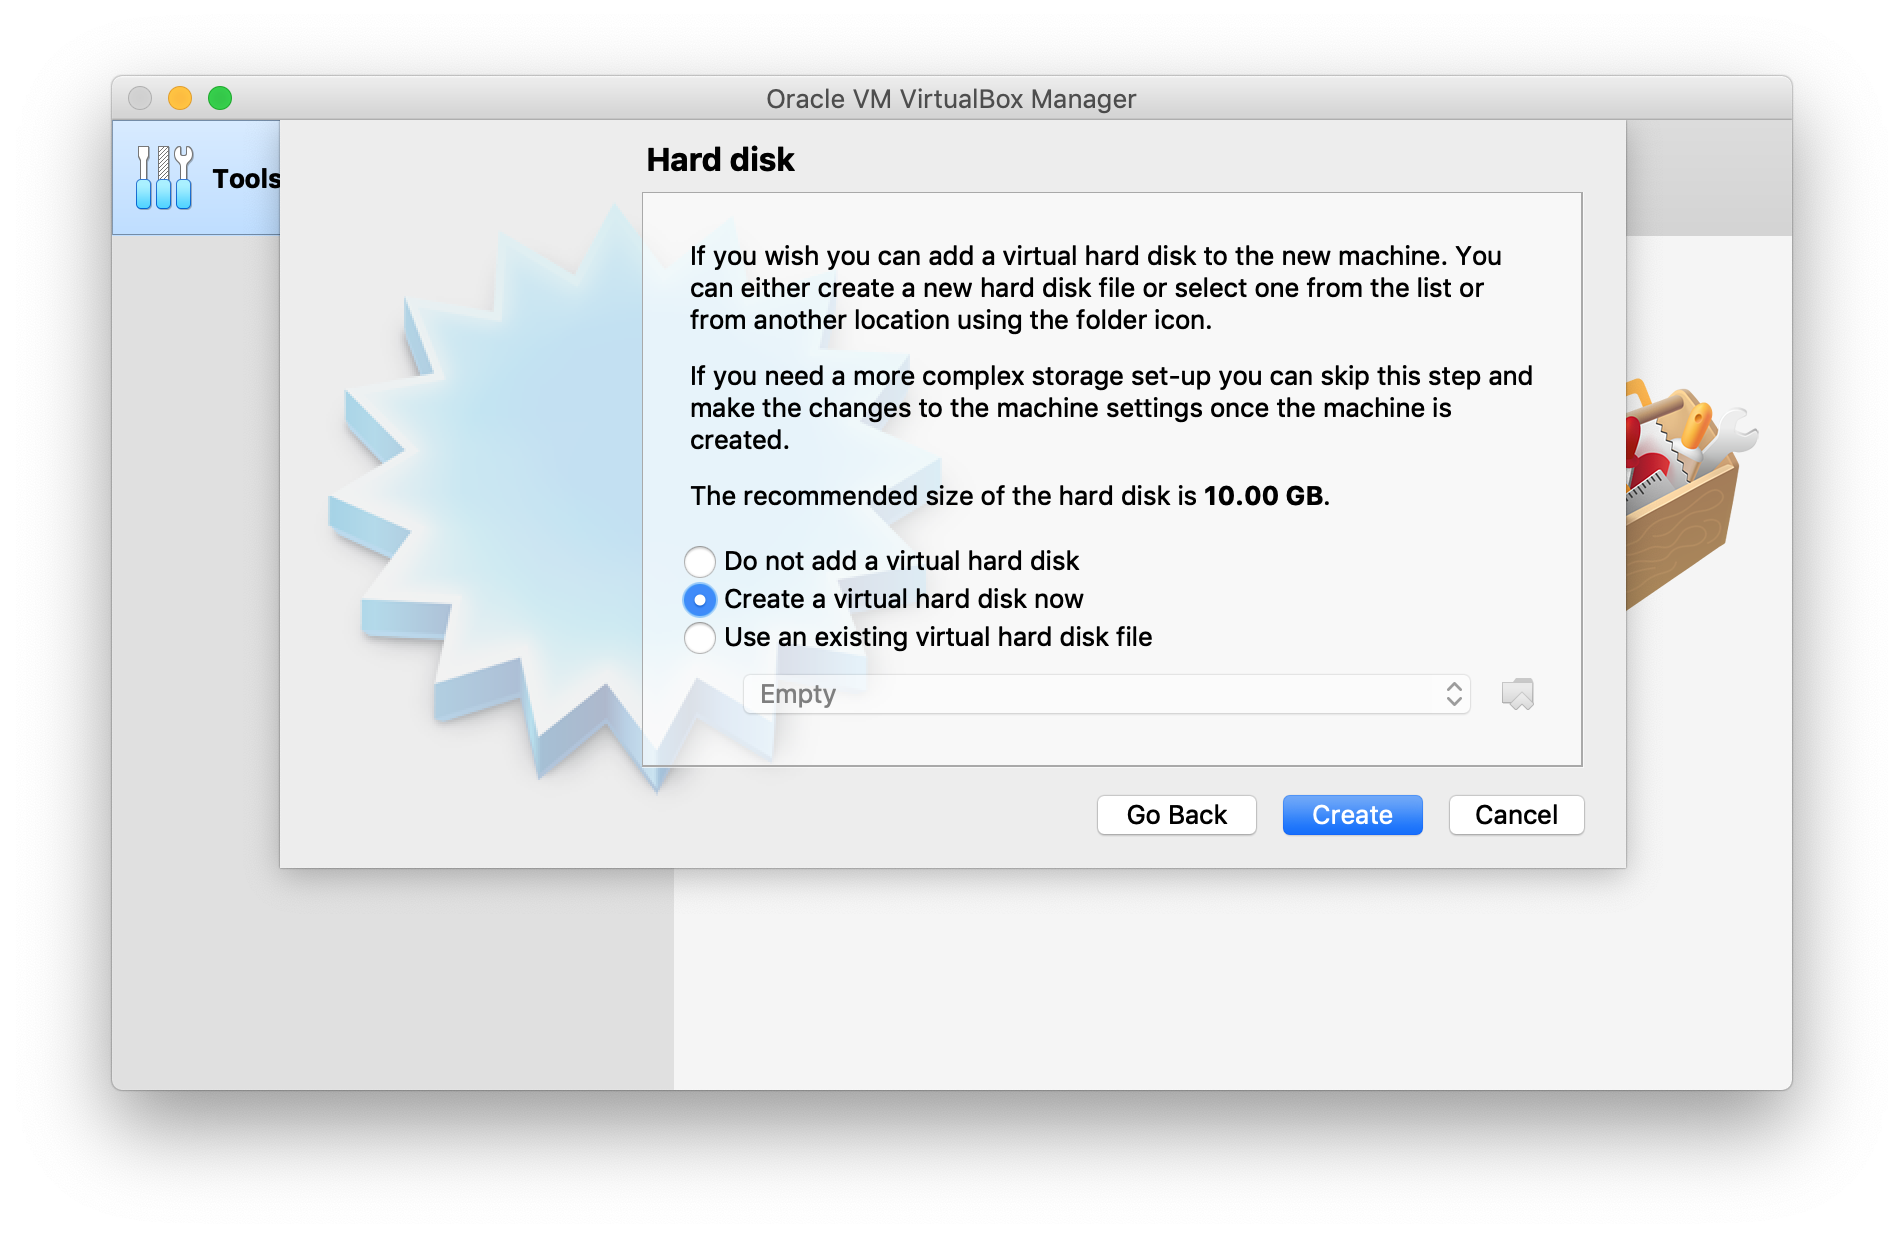
\includegraphics[width=0.8\linewidth]{vb-hd}
  \end{center}
  Our virtual machine also needs a virtual hard disk
\end{frame}

\begin{frame}{Create Virtual Hard Disk (2/4)}
  \begin{center}
    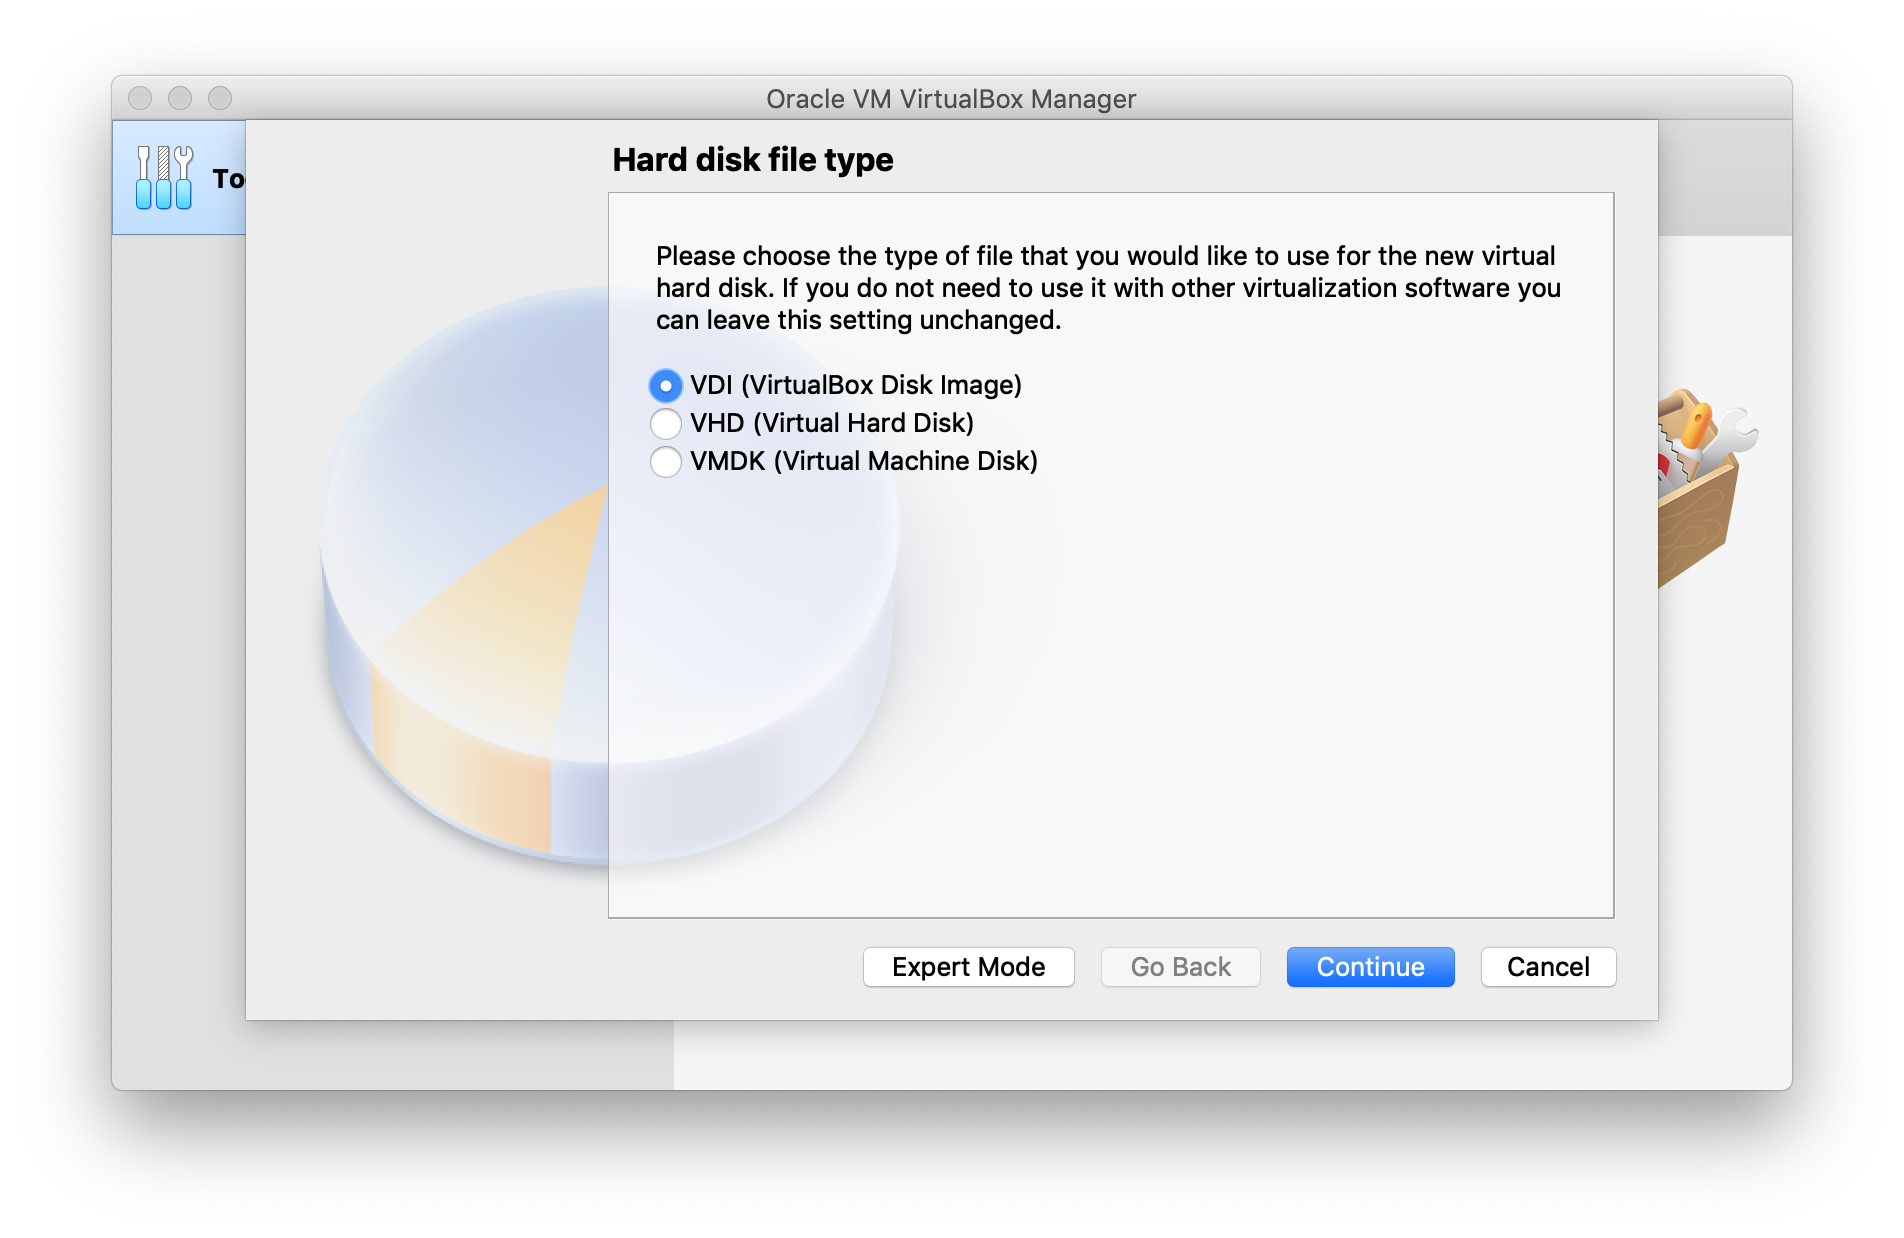
\includegraphics[width=0.8\linewidth]{vb-hd2}
  \end{center}
  Use the default virtual HD format for best performance.
\end{frame}

\begin{frame}{Create Virtual Hard Disk (3/4)}
  \begin{center}
    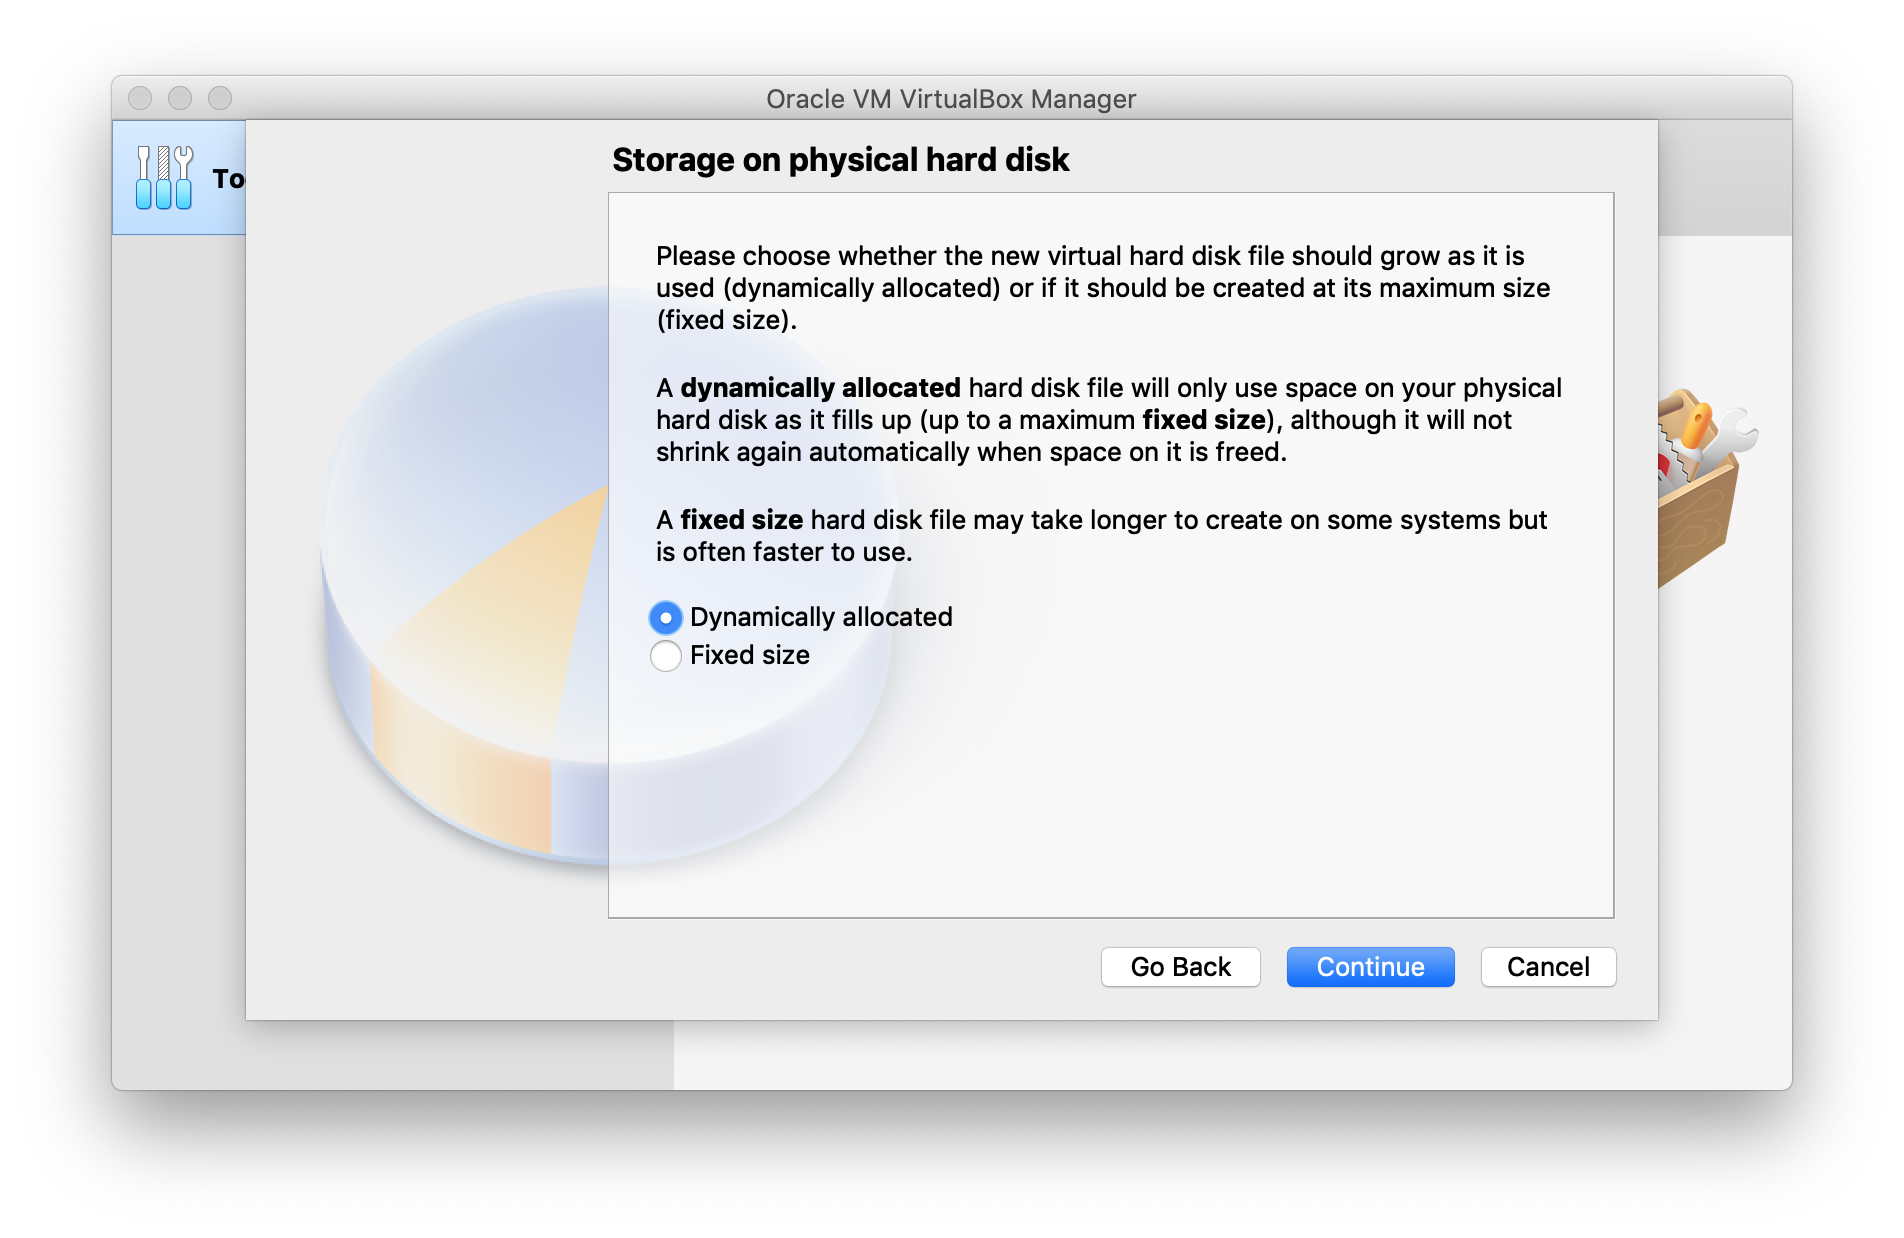
\includegraphics[width=0.8\linewidth]{vb-hd3}
  \end{center}
  Keep it dynamically-sized so the virtual HD will only take up as much space as it currently needs.
\end{frame}

\begin{frame}{Create Virtual Hard Disk (4/4)}
  \begin{center}
    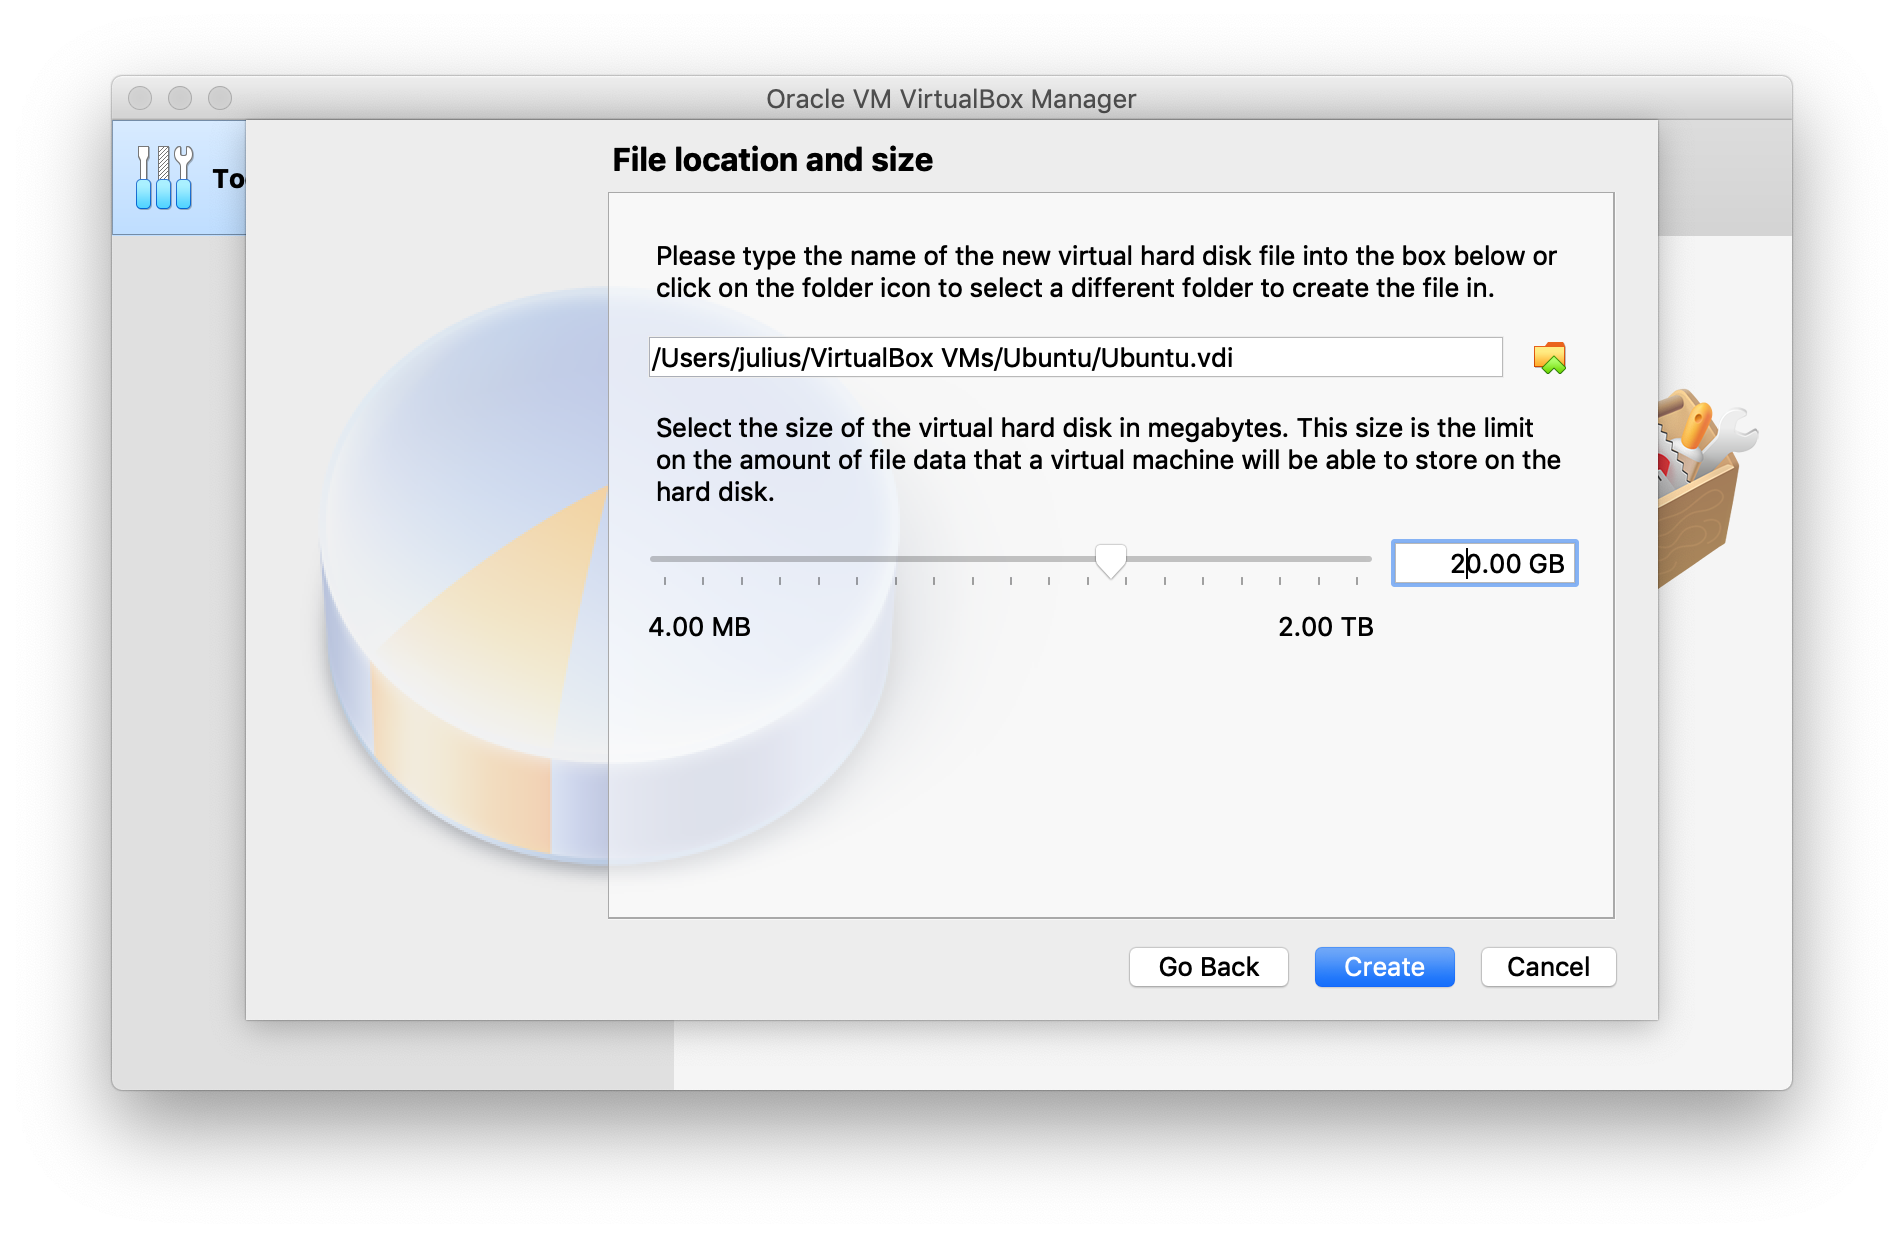
\includegraphics[width=0.8\linewidth]{vb-hd4}
  \end{center}
  Ubuntu has a minimum of 10 GiB and recommends 25 GiB. In any case, we will be using the minimum installation, amounting to about 6 GiB.
\end{frame}

\begin{frame}{Back to the main UI}
  \begin{center}
    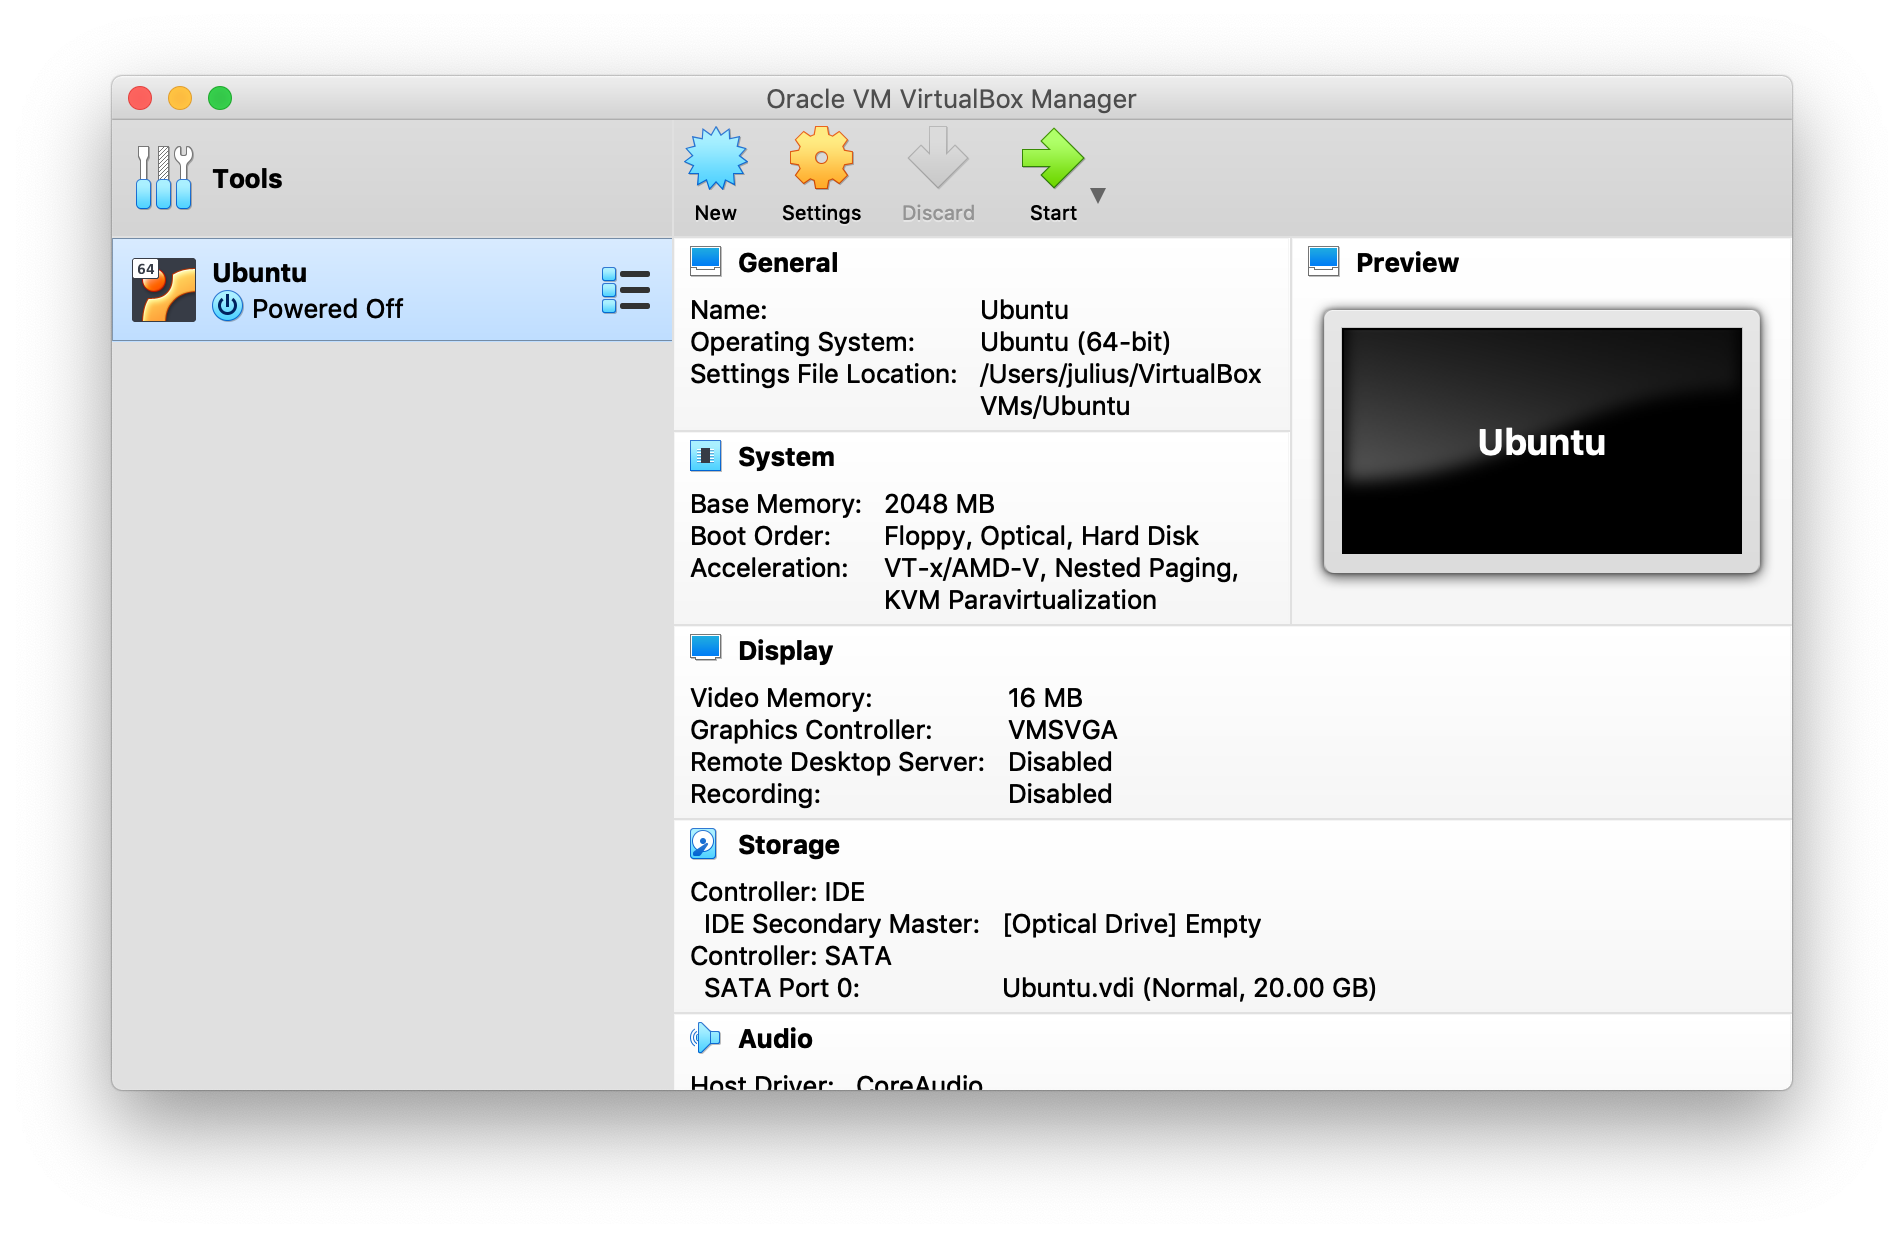
\includegraphics[width=0.8\linewidth]{vb-main2}
  \end{center}
  Click on ``Settings''
\end{frame}

\begin{frame}{Settings}
  \begin{center}
    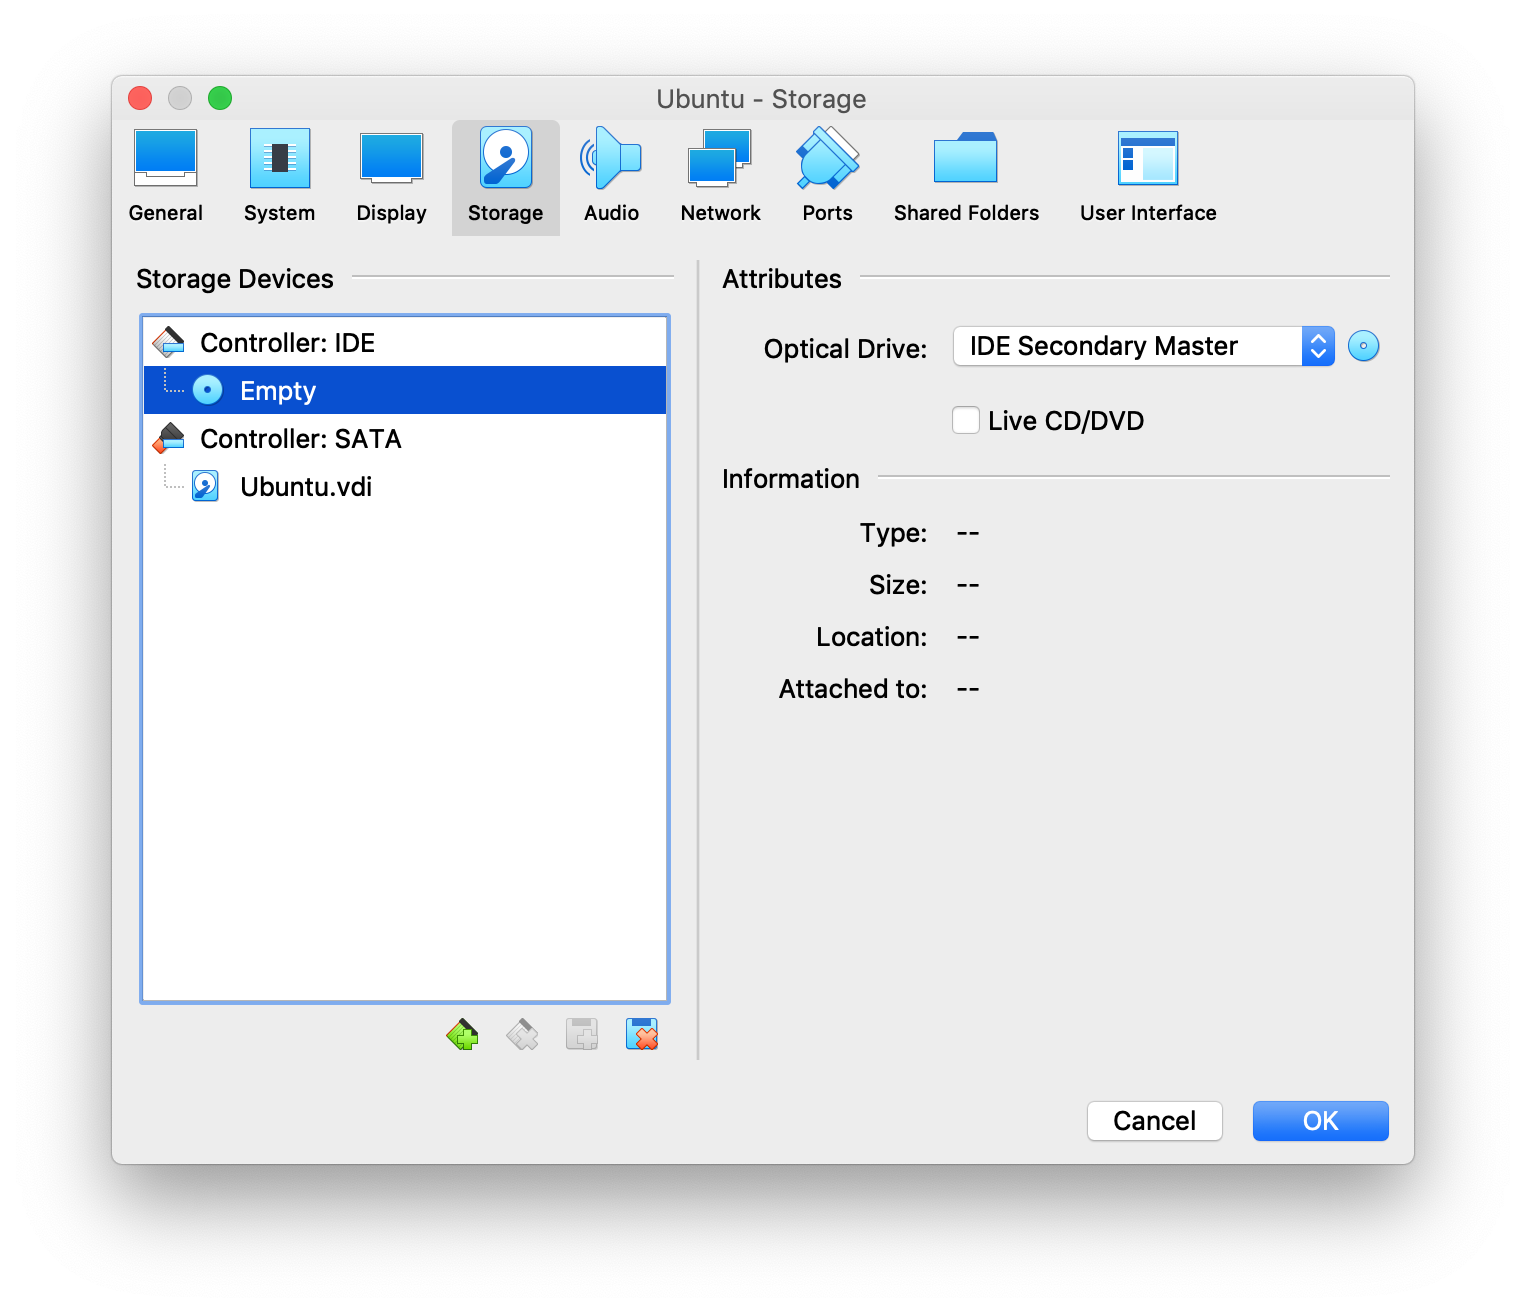
\includegraphics[width=0.8\linewidth]{vb-settings}
  \end{center}
  Go to ``Storage'', then on the Empty in Controller: IDE. Click on the disc button beside ``IDE Secondary Master'', then ``Choose Virtual Optical Disk File''
\end{frame}

\begin{frame}{Choose Disc}
  \begin{center}
    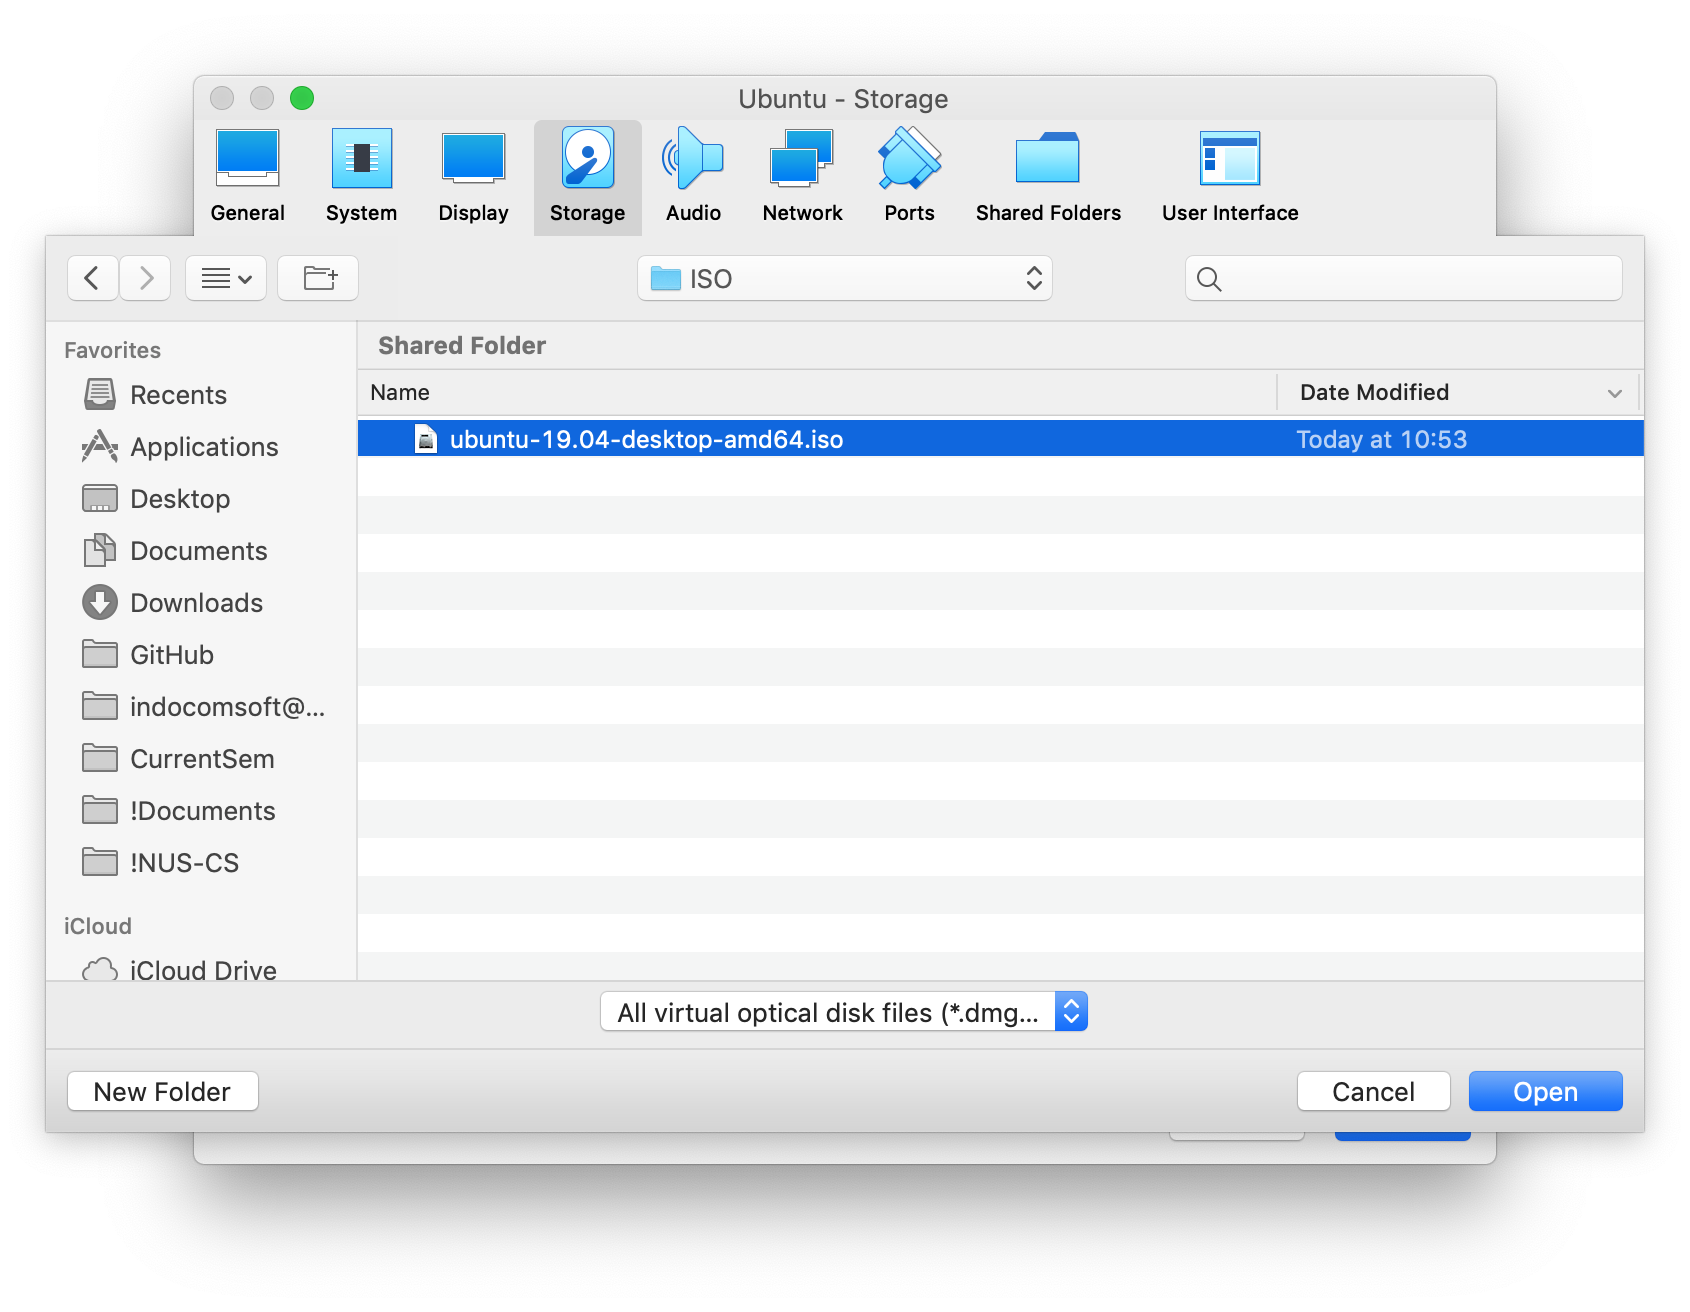
\includegraphics[width=0.7\linewidth]{vb-disc}
  \end{center}
  Choose your Ubuntu ISO file
\end{frame}

\begin{frame}{Finally}
  We are done with the VirtualBox set-up!

  Feel free to go to settings later on and customise to your heart's desire.

  For now, you can click ``Start'' in the main UI.
\end{frame}

\section{Linux Install Fest}
\subsection{}

\begin{frame}{Booting Ubuntu}
  \begin{columns}
    \begin{column}{0.65\linewidth}
      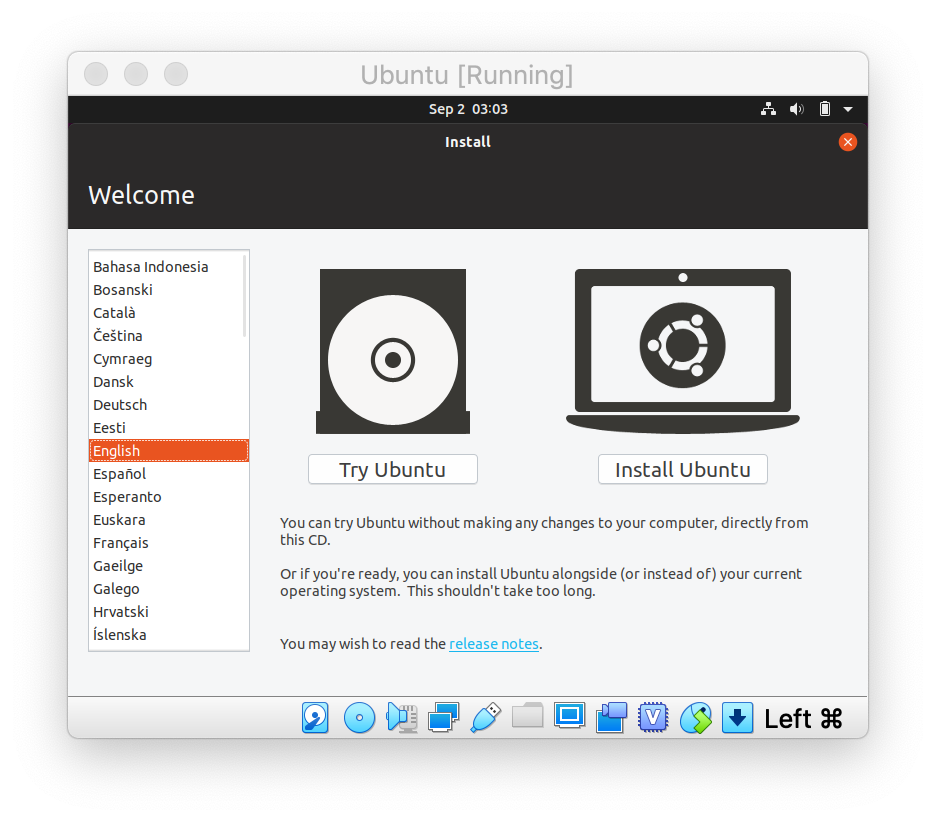
\includegraphics[width=\linewidth]{ubuntu}
    \end{column}
    \begin{column}{0.35\linewidth}
      Once the VM starts and boots, you should see this screen.

      Choose ``Install Ubuntu''
    \end{column}
  \end{columns}
\end{frame}

\begin{frame}{Choose Keyboard Layout}
  \begin{columns}
    \begin{column}{0.65\linewidth}
      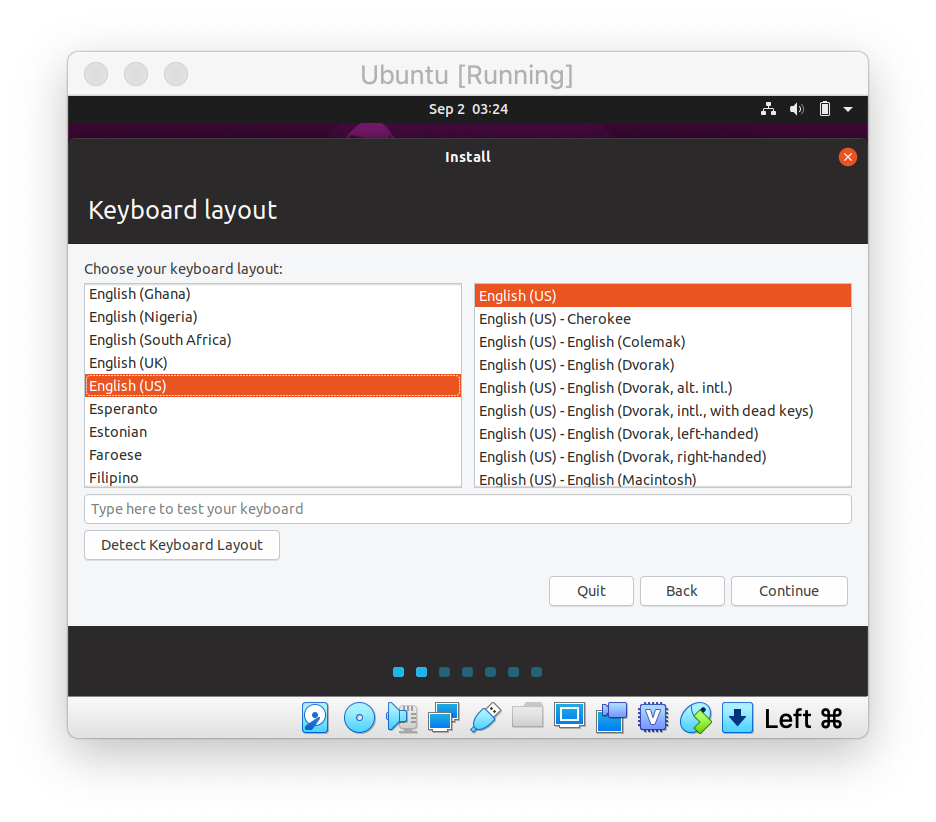
\includegraphics[width=\linewidth]{ubuntu-kb}
    \end{column}
    \begin{column}{0.35\linewidth}
      Choose your keyboard layout. Most computers sold in Singapore use English (US).
    \end{column}
  \end{columns}
\end{frame}

\begin{frame}{Updates and Other Software}
  \begin{columns}
    \begin{column}{0.65\linewidth}
      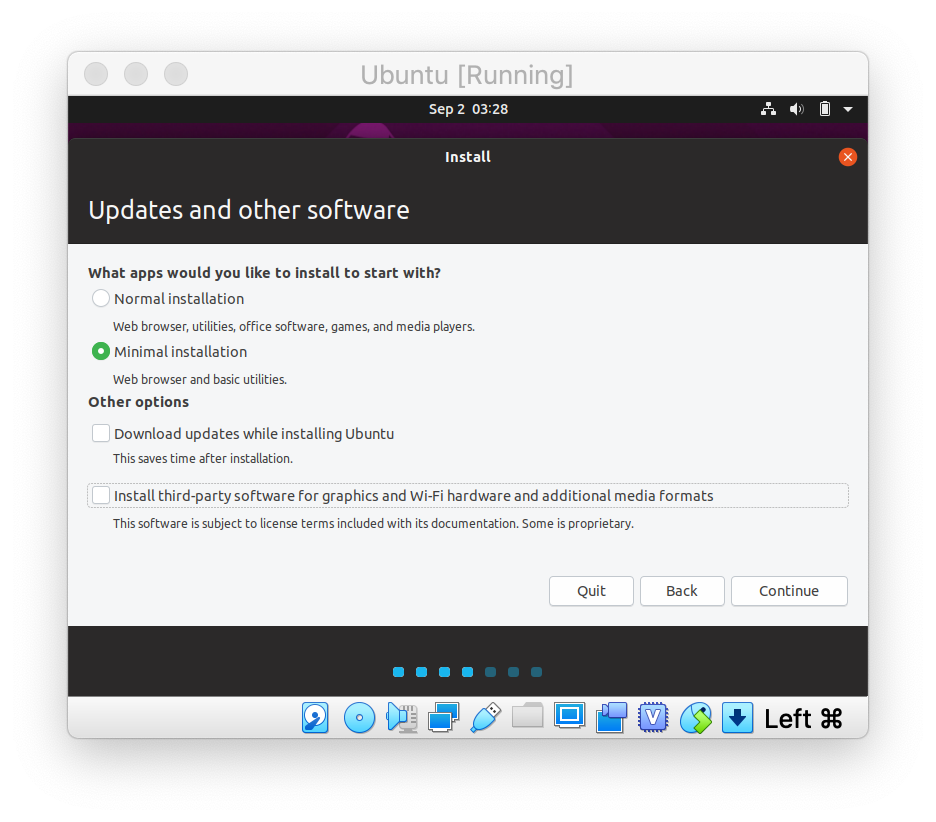
\includegraphics[width=\linewidth]{ubuntu-update}
    \end{column}
    \begin{column}{0.35\linewidth}
      Choose minimal installation, and do not tick the checkboxes to save time on instalattion.
    \end{column}
  \end{columns}
\end{frame}

\begin{frame}{Installation Type}
  \begin{columns}
    \begin{column}{0.65\linewidth}
      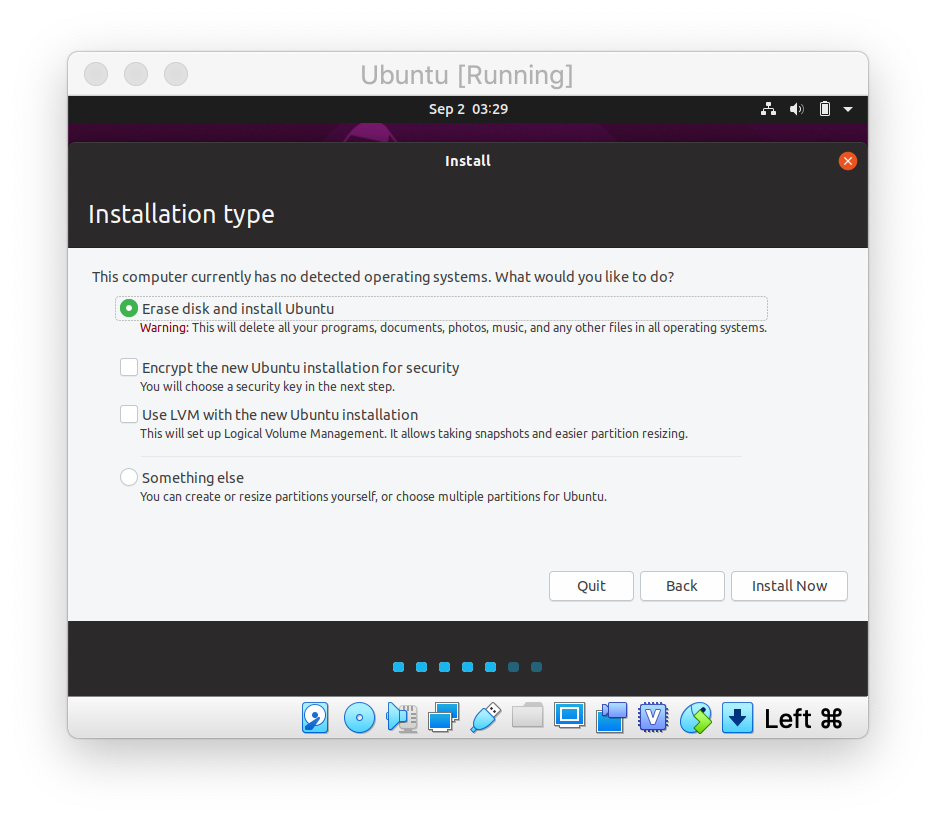
\includegraphics[width=\linewidth]{ubuntu-disk}
    \end{column}
    \begin{column}{0.35\linewidth}
      Choose ``Erase disk and install ubuntu'', then ``Install now''. Click ``Continue'' on the dialogue that shows up.
    \end{column}
  \end{columns}
\end{frame}

\begin{frame}{Location}
  \begin{columns}
    \begin{column}{0.65\linewidth}
      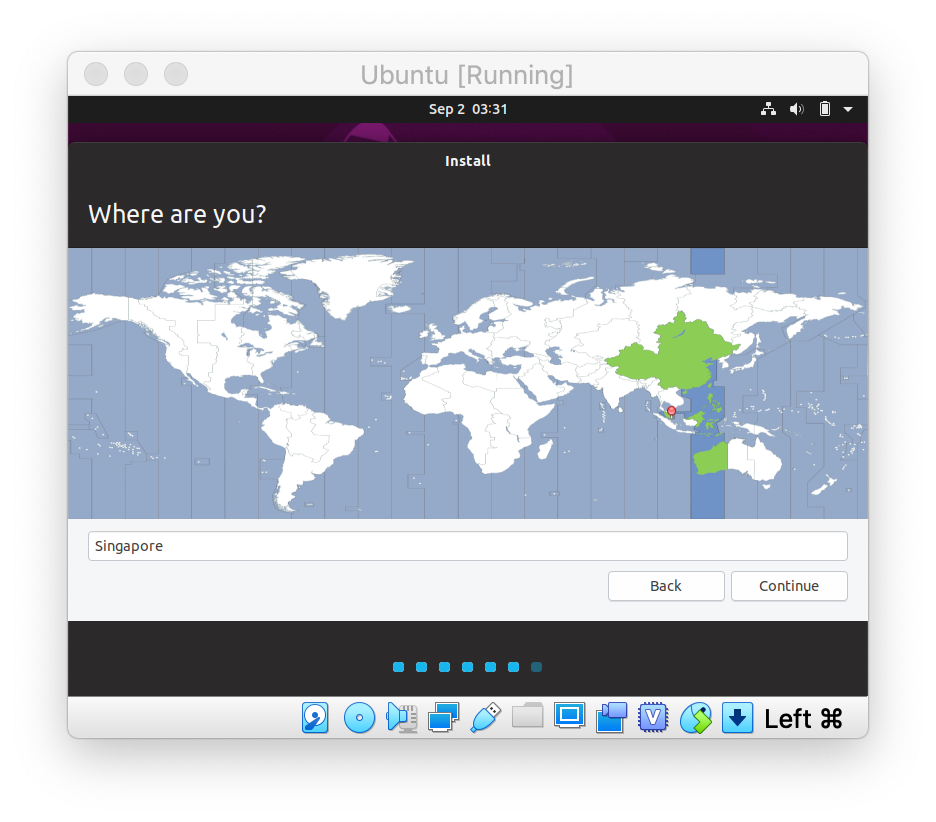
\includegraphics[width=\linewidth]{ubuntu-tz}
    \end{column}
    \begin{column}{0.35\linewidth}
      Ubuntu should already detect that you're in Singapore.
    \end{column}
  \end{columns}
\end{frame}

\begin{frame}{Setting up username}
  \begin{columns}
    \begin{column}{0.65\linewidth}
      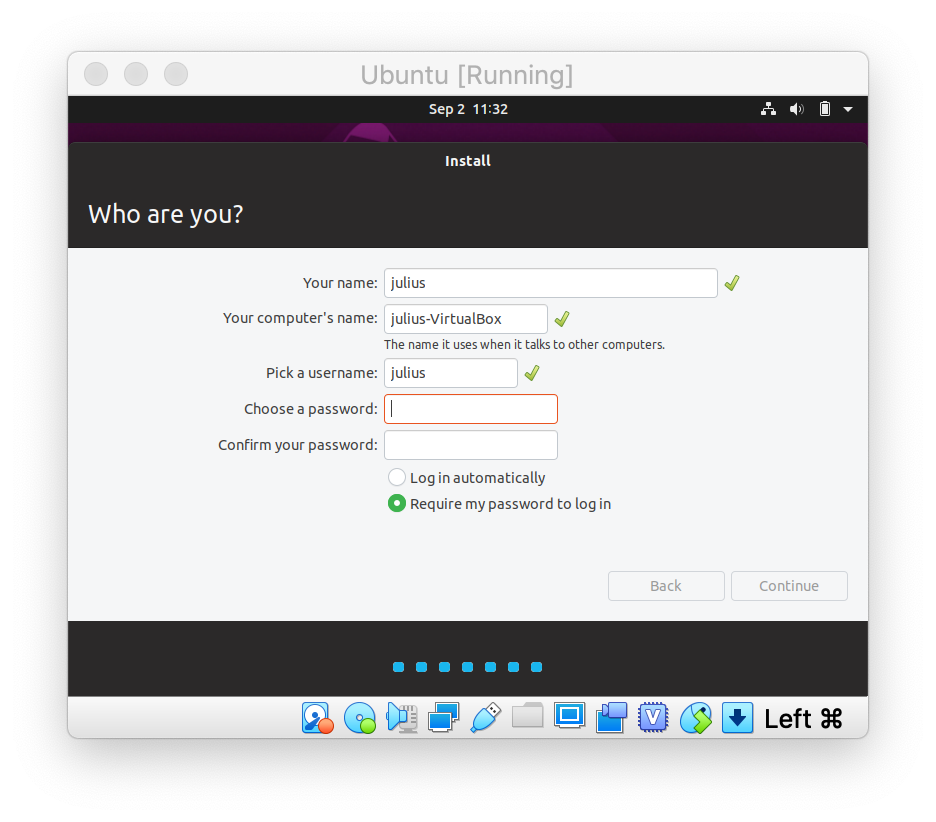
\includegraphics[width=\linewidth]{ubuntu-user}
    \end{column}
    \begin{column}{0.35\linewidth}
      Type in your name, and set a password.
    \end{column}
  \end{columns}
\end{frame}

\begin{frame}{Sit back and relax}
  \begin{center}
    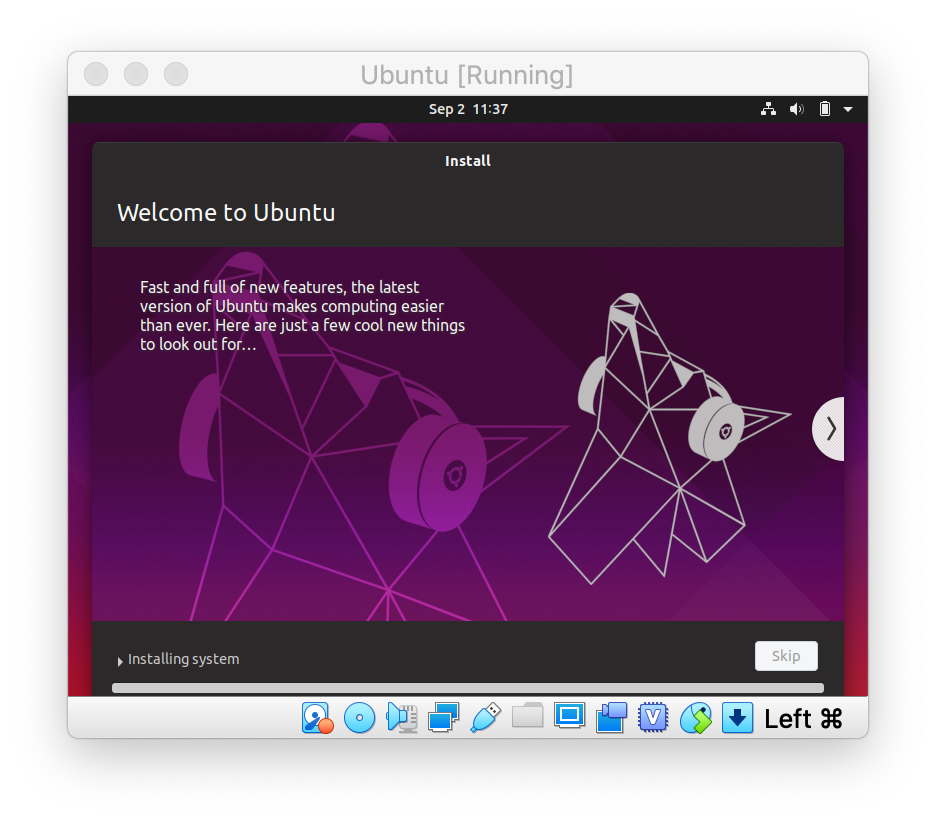
\includegraphics[width=0.8\linewidth]{ubuntu-installing}
  \end{center}
\end{frame}

\section{Nifty Tricks with VM}
\subsection{Force shutdown the VM}
\begin{frame}{Force Shutdown the VM}
  You may need to run unstable software on the VM.

  If the VM hangs, you can always force shutdown by closing and choosing ``Power off the machine'', and quickly bring up the VM again.
\end{frame}

\subsection{Saving State \& Snapshot}
\begin{frame}{Saving machine state}
  You need not shut down the OS to shut down your VM.

  Instead, you can just save its state and ``pause'' the VM, to be resumed later.

  Try closing the VM, and choose ``Save the machine state''
\end{frame}

\begin{frame}{What is Snapshot?}
  Captures the state of the VM at one particular time.

  You can always get back to this state later on.

  Useful for experimentation!
\end{frame}

\begin{frame}{Taking Snapshot in VirtualBox}
  \menu{Machine > Take Snapshot}
  \begin{center}
    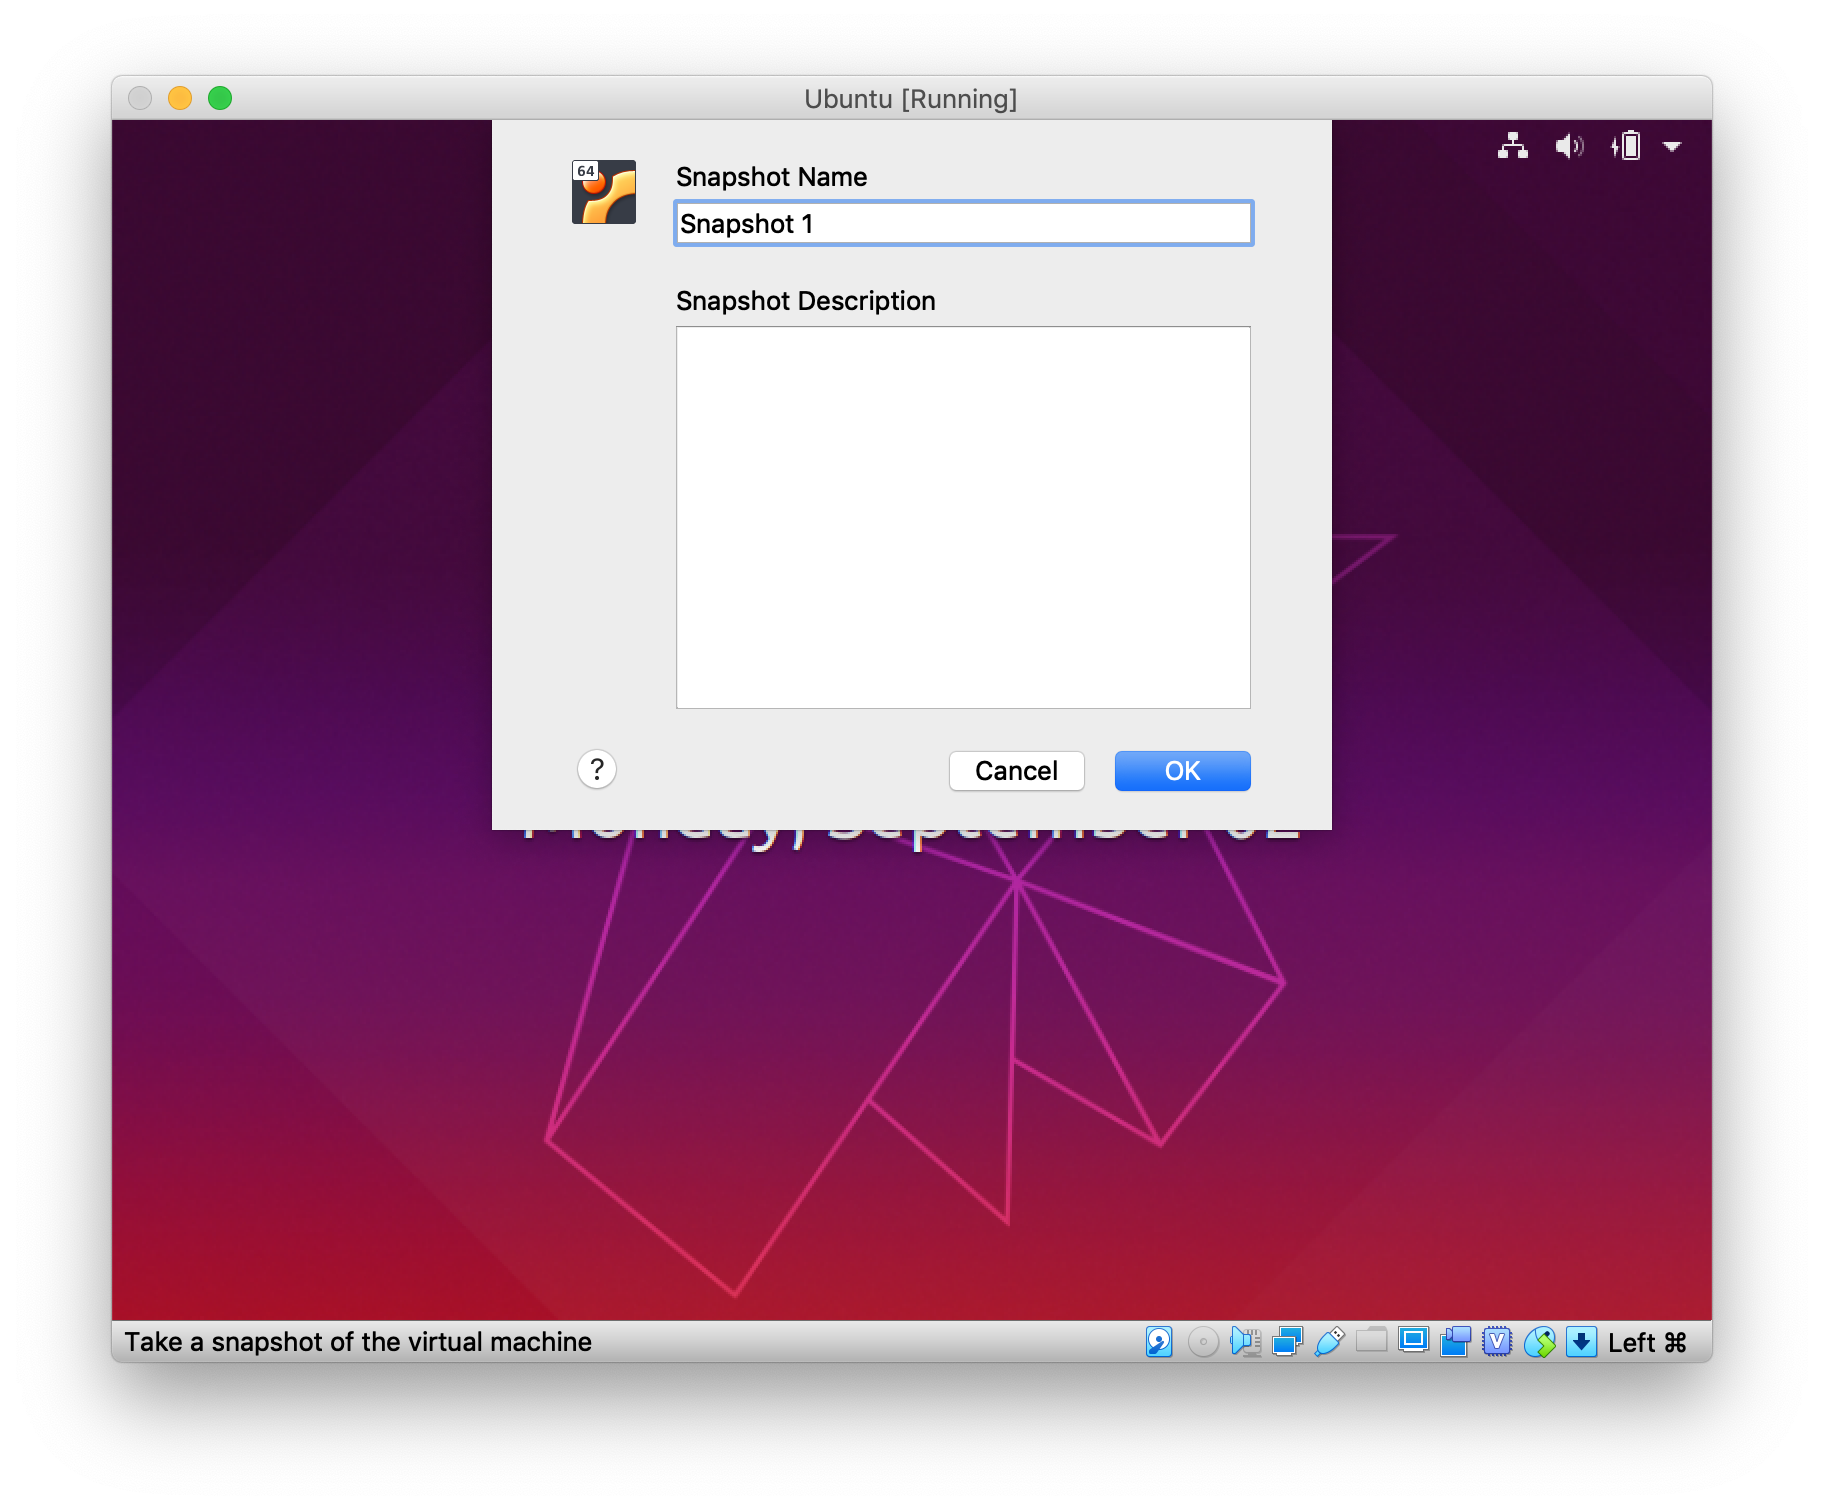
\includegraphics[width=0.7\linewidth]{snapshot}
  \end{center}
\end{frame}

\begin{frame}{See List of Snapshot in VirtualBox}
  On the main UI of VirtualBox, click the list icon besides the VM name (Ubuntu) and select ``Snapshots''
  \begin{center}
    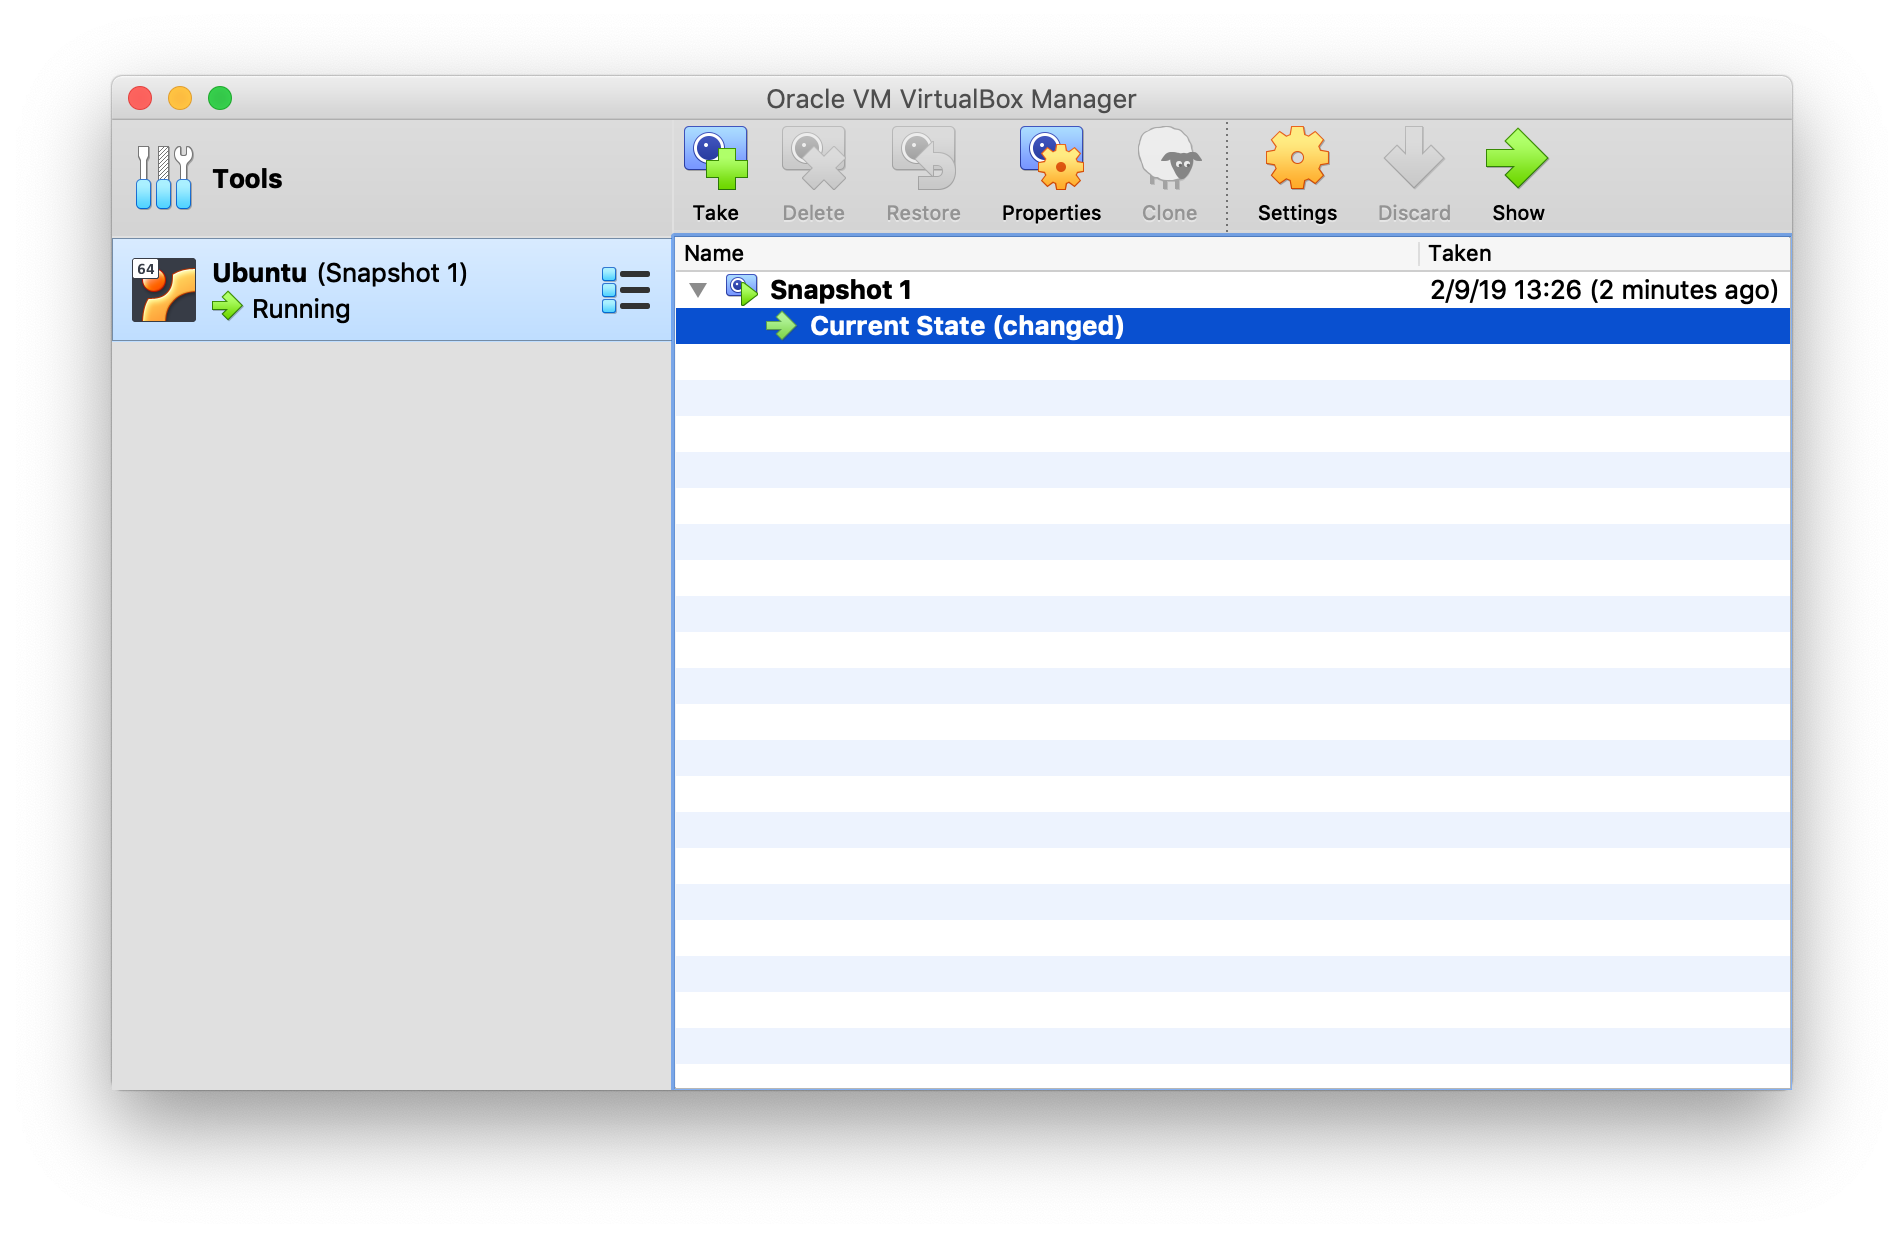
\includegraphics[width=0.8\linewidth]{vb-snapshots}
  \end{center}
\end{frame}

\begin{frame}{Restoring Snapshot in VirtualBox}
  To restore, your VM must be shut down.

  In this case, we don't really care about the current state, so either shut down the OS, or close the VM and choose ``Power off the machine''

  In the list of snapshots, select the snapshot to restore, and click ``Restore''
\end{frame}

\subsection{Go crazy and experiment!}
\begin{frame}[fragile]{Some risky things to do}
  Open up the terminal (shortcut: \keys{\ctrlwin + \Altwin + t}) and figure out what these commands do and try them out:

  \mintinline{bash}{sudo rm -rf --no-preserve-root /}

  \mintinline{bash}{:(){:|:&};:}
\end{frame}

\subsection{Guest Addons}
\begin{frame}{Guest Addons}
  VMs actually provide some software for better integration, e.g. shared clipboard, screen auto-resizing, etc.

  In VirtualBox, this is called the Guest Additions.
\end{frame}

\begin{frame}{Installing VirtualBox Guest Additions}
  \menu{Devices > Insert Guest Additions CD Image}

  This will insert the Guest Additions as a virtual CD.

  Choose ``Run''
\end{frame}

\section{Conclusion}
\subsection{}
\begin{frame}
  \frametitle{Talk to us!}
  \begin{itemize}
    \item \textbf{Feedback form}: \url{https://is.gd/2019ht4}
    \item \textbf{Upcoming Hacker Tools}:

          Shell \& Scripting, SR10, 10th September 2019, 6.30pm
  \end{itemize}
\end{frame}

\end{document}
